%%%%%%%%%%%%%%%%%%%%%%%%%%%%%%%%%%%%%%%%%%%%%%%%%%%%%%%%%%%%%%%%%%%%%%%%
%                                                                      %
% LaTeX, FIIW thesis template                                          %
% 28/11/2014 v1.2                                                      %
%                                                                      %
%%%%%%%%%%%%%%%%%%%%%%%%%%%%%%%%%%%%%%%%%%%%%%%%%%%%%%%%%%%%%%%%%%%%%%%%
\documentclass[11pt,a4paper]{report}
% Indien je je thesis recto-verso wil afdrukken gebruik je onderstaande opties i.p.v. bovenstaande
%\documentclass[11pt,a4paper,twoside,openright]{report}

\usepackage[a4paper,left=3.5cm, right=2.5cm, top=3.5cm, bottom=3.5cm]{geometry}
\usepackage[dutch]{babel}
\usepackage{graphicx}
\usepackage[latin1]{inputenc}           % om niet ascii karakters rechtstreeks te kunnen inputten
%\usepackage[utf8]{inputenc}            % commentarieer deze regel uit als je utf8 encoded files gebruikt in plaats van latin1
\usepackage{natbib}
\usepackage{listings}             		% voor het weergeven van broncode
\usepackage{verbatim}					% weergeven van code, commando's, ...
\usepackage{hyperref}					% maak PDF van de thesis navigeerbaar
\usepackage{url}						% URL's invoegen in tekst met behulp van \url{http://}
\usepackage[small,bf,hang]{caption}     % om de captions wat te verbeteren
\usepackage[final]{pdfpages}            % gebruikt voor het invoegen van het artikel in pdf-formaat
\usepackage{pslatex}					% andere lettertype's dan de standaard types

\usepackage{sectsty}					% aanpassen van de fonts van sections en chapters
\allsectionsfont{\sffamily}
\chapterfont{\sffamily}

\usepackage{float}                      % De optie H voor de plaatsing van figuren op de plaats waar je ze invoegt. bvb. \begin{figure}[H]
%Eigen packages
\usepackage[dutch]{varioref}
\usepackage{graphicx}
\usepackage{rotating}
\usepackage{amsmath}
\usepackage{booktabs}
\usepackage{slashbox}
%\usepackage{longtable}					% tabellen die over meerdere pagina's gespreid worden
%\usepackage[times]{quotchap}           % indien je fancy hoofdstuktitels wil
%\usepackage[none]{hyphenat}
%\usepackage{latexsym}
%\usepackage{amsmath}
%\usepackage{amssymb}
\usepackage{fiiw_gent}
% \usepackage{fiiw_ghent_eng} % For the english version (also change last page at the bottom of this file!

%door onderstaande regels in commentaar te zetten, of op false, kan je pagina's weglaten
%bijvoorbeeld het weglaten van een voorwoord, lijst met symbolen, ...
%%%%%%%%%%%%%%%%%%%%%%%%%%%%%%%%%%%%%%%%%%%%%%%%%%%%%%%%%%%%%%%%%%%%%%%%%%%%%%%%%%%%%%%%
%voorwoord toevoegen?
%\acknowledgementspagetrue
%\acknowledgements{voorwoord}			%.tex file met daarin het voorwoord
%abstract toevoegen?
%\abstractpagetrue
%\abstracts{abstract}					%.tex file met daarin het abstract
%lijst van figuren toevoegen?
%\listoffigurespagetrue
%lijst van tabellen toevoegen?
%\listoftablespagetrue
%lijst van symbolen toevoegen?
%\listofsymbolspagetrue
%\listofsymbols{symbolen}				%.tex file met daarin de lijst van symbolen

%informatie over het eindwerk, de promotor, ...
%%%%%%%%%%%%%%%%%%%%%%%%%%%%%%%%%%%%%%%%%%%%%%%
\opleiding{Industri\"ele ingenieurswetenschappen}
\afdeling{Elektronica-ICT: Elektronica}

\title{Ontwikkeling van een\\autonoom lijn-volgend\\racevoertuig}
\subtitle{}
\forenameA{Jorik}
\surnameA{De Bruycker}
\forenameB{Jonas}
\surnameB{Bolle}
\academicyear{2017 - 2018}

\promotorA[Begeleiders]{Leenders Guus\\Crul Stijn\\Naessens Carine\\Van der Perre Liesbet}
\promotorB[Coach]{Cox Bert}

\begin{document}
\selectlanguage{dutch}
\preface
\tableofcontents

\chapter{Inleiding}\label{sec:inleiding}
\section{Opdrachtbeschrijving}
In het kader van ons bachelorproject ontwikkelen we een wagentje dat autonoom zo snel mogelijk een raceparcours kan afleggen. Dit parcours bestaat uit een zwarte ondergrond afgebakend door volle witte lijnen en een witte stippellijn in het midden, een voorbeeld hiervan ziet u in figuur~\vref{fig:parcoursvoorbeeld}. Ons wagentje mag niet buiten de volle witte lijnen van het parcours treden. Tevens zullen er op het traject verschillende RFID-tags geplaatst worden die door het voertuig ingelezen moeten worden. Eveneens moet er een manier voorzien worden om de snelheid van het voertuig te meten. De ingelezen tags en opgemeten snelheid moet ten slotte nog verzonden worden naar een Raspberry Pi. Voor het aanschaffen van nodige hardware krijgen we 50 euro ter beschikking.\\
\begin{figure}[H]
	\centering
	\includegraphics[width=\textwidth]{parcoursvoorbeeld.png}
	\caption{Voorbeeld parcours dat ons wagentje dient af te leggen}
	\label{fig:parcoursvoorbeeld}
\end{figure}
\subsection{Hardware}
We krijgen reeds een wagentje met twee motoren en een batterij om te beginnen.
Voor het prototypen en testen mogen we gebruik maken van een Arduino Uno met motor shield, een belangrijk deel van de opdracht bestaat er uit deze Arduino \'en motor shield te vervangen door \'e\'en custom board.
Qua hardware moeten we dus nog de custom board ontwikkelen, sensoren voorzien en uiteraard ook modules aanschaffen voor (Bluetooth) communicatie met de RPi en het inlezen van RFID-tags.\\
\subsection{Software}
De besproken hardware moet natuurlijk ook correct aangestuurd worden door software. Dit zal gebeuren aan de hand van Arduino-code ondersteund door C/C++ libraries. In deze software moeten voorzieningen getroffen worden voor het aansturen van de motoren, het inlezen van sensoren, communicatie met Raspberry Pi,...
Aan de kant van de Raspberry Pi zullen we verbinding moeten maken met ons wagentje en de data die doorgestuurd wordt af printen op het scherm.


\section{Doelstellingen}
De belangrijkste doelstellingen van ons project zijn dus de volgende:
\begin{itemize}
	\item Voertuig autonoom en zo snel mogelijk een parcours laten afleggen
	\item Custom board ontwerpen om Arduino en motorshield te vervangen
	\item Snelheid van het wagentje meten
	\item RFID-lezer voorzien voor het uitlezen van tags op het parcours
	\item Communicatie (Bluetooth) tussen Arduino en Raspberry Pi 3 realiseren
\end{itemize}
\section{Structuur}
We beginnen dit verslag met een bespreking van onze planning, taakverdeling en gemaakte onkosten. Daarna behandelen we de gebruikte hardware en software om deze aan te sturen in meer detail. Vervolgens overleggen we de problemen en moeilijkheden die we doorheen het project ondervonden. Hierna volgt nog een evaluatie van onze coach, Bert Cox. Ten slotte eindigen we met een besluit omtrent het project waarin we samenvatten wat we gerealiseerd hebben, wat we hebben bijgeleerd, wat er beter kan/kon,...
\chapter{Taakverdeling}\label{sec:taakverdeling}
\begin{table}[H]
	\setlength\aboverulesep{0pt}
	\setlength\belowrulesep{0pt}
	\renewcommand{\arraystretch}{3}
	\centering
	\resizebox{\textwidth}{!}{%
		\begin{tabular}{@{}|c|c|c|c|@{}}
			\toprule
			\multicolumn{2}{|c|}{\textbf{\backslashbox{Periode}{Groepslid}}} & \textbf{Bolle Jonas}                          & \textbf{De Bruycker Jorik}                           \\ \midrule
			\textbf{nov}                  & \textbf{jan}                & \multicolumn{2}{c|}{Ori\"enteren omtrent opdracht, overleggen van idee\"en, voorbereidend opzoekwerk}                                                        \\
			\midrule
			\textbf{1/feb}                  & \textbf{11/feb}                & \multicolumn{2}{c|}{Bestellen benodigdheden, concrete afspraken, aanvang project}                                                        \\ \midrule
			\textbf{12/feb}                 & \textbf{25/feb}                & Custom Arduino: research & Ontwerp IR-sensorarrays                              \\ \midrule
			\textbf{26/feb}                 & \textbf{11/mrt}                & Custom Arduino: Eagle schematic               & Start software sensoren en bijsturen                 \\ \midrule
			\textbf{12/mrt}                 & \textbf{25/mrt}                & Custom Arduino: Eagle routing                 & Software PID-regeling                                \\ \midrule
			\multicolumn{2}{|c|}{\textbf{21/mrt}}                            & \multicolumn{2}{c|}{Eerste statusupdate}                                                             \\ \midrule
			\textbf{26/mrt}                 & \textbf{1/apr}                 & Custom Arduino: etsen                         & Snelheidsmeter voorzien                              \\ \midrule
			\textbf{2/apr}                  & \textbf{15/apr}                & Custom Arduino: bestukken, solderen en testen & Bluetooth-communicatie met RPi3, RFID-lezer voorzien \\ \midrule
			\textbf{16/apr}                 & \textbf{27/apr}                & \multicolumn{2}{c|}{Verslag schrijven}                                                               \\ \midrule
			\multicolumn{2}{|c|}{\textbf{18/apr}}                            & \multicolumn{2}{c|}{Demonstratie/race}                                                               \\ \midrule
			\multicolumn{2}{|c|}{\textbf{27/apr}}                            & \multicolumn{2}{c|}{Verslag indienen}                                                                \\ \midrule
			\textbf{28/apr}                 & \textbf{8/mei}                 & \multicolumn{2}{c|}{Presentatie voorbereiden}                                                        \\ \midrule
			\multicolumn{2}{|c|}{\textbf{9/mei}}                             & \multicolumn{2}{c|}{Presentatie}                                                                     \\ \bottomrule
		\end{tabular}%
	}
	\caption{Planning en taakverdeling}
	\label{table:planning}
\end{table}
\chapter{Onkosten}\label{sec:onkosten}
We kregen voor dit project een bedrag van 50 euro ter beschikking.
Onze uitgaven van dit budget kan u vinden in tabel~\vref{table:onkosten}. In totaal komt dit neer op een bedrag van 21,72 euro.  

\begin{table}[H]
\renewcommand{\arraystretch}{2}
\centering
\begin{tabular}{llll}
order nr. + beschrijving                                                           & prijs/stuk (euro)          & aantal                  & totaal (euro)             \\ \hline
\multicolumn{1}{|l|}{1703519: TCRT5000L infrarood sensor}                          & \multicolumn{1}{l|}{0.741} & \multicolumn{1}{l|}{10} & \multicolumn{1}{l|}{7.41} \\ \hline
\multicolumn{1}{|l|}{1470593: SS41 hall sensor}                                    & \multicolumn{1}{l|}{0.88}  & \multicolumn{1}{l|}{6}  & \multicolumn{1}{l|}{5.28} \\ \hline
\multicolumn{1}{|l|}{1106109: CD4051BE 8:1 analog multiplexer}                     & \multicolumn{1}{l|}{0.415} & \multicolumn{1}{l|}{5}  & \multicolumn{1}{l|}{2.08} \\ \hline
\multicolumn{1}{|l|}{1703519: TCRT5000L infrarood sensor (later extra bijbesteld)} & \multicolumn{1}{l|}{0.695} & \multicolumn{1}{l|}{10} & \multicolumn{1}{l|}{6.95} \\ \hline
\end{tabular}
\caption{Onkosten}
\label{table:onkosten}
\end{table}

Andere vereisten zoals de Bluetooth-module en RFID-lezer werden voorzien zonder zelf te bestellen.
\chapter{Toelichting hardware}\label{sec:toelichting-hardware}
In dit hoofdstuk bekijken we de gebruikte hardware meer in detail. We bespreken eerst het ontwerp van ons custom Arduino board. Vervolgens gaan we dieper in op de gebruikte sensoren en modules. Ten slotte halen we kort enkele eigenschappen van de Raspberry Pi aan die voor ons relevant zijn.

\section{PCB-ontwerp}
Voor het ontwerp van de custom Arduino PCB hebben we gewerkt met Eagle. Vertrekkende van de offici\"{e}le schematic van de Arduino Uno maken we onze eigen versie hiervan. Na de ontwerpfase kunnen we de PCB etsen, boren, bestukken en solderen. Als dit allemaal achter de rug is, testen we onze custom Arduino en lossen we nog eventuele problemen op. 
\subsection{Eagle-ontwerp}
\subsubsection{Schematic}
Om onze custom board te ontwerpen moeten we uiteraard niet helemaal vanaf nul beginnen. We vertrokken van het offici\"{e}le schema dat makkelijk online te vinden is (zie figuur~\vref{fig:ardsch}). We bestudeerden dit schema grondig om te bepalen welke componenten we effectief nodig hebben en welke we weg kunnen laten. Hieruit bleek dat er veel onderdelen uit het originele ontwerp niet vereist zijn voor onze doeleinden. Zoals bijvoorbeeld de USB to serial interface, aangezien we beslisten om onze custom Arduino te programmeren via de ICSP-pinnen, is de aanwezigheid van een USB-connectie overbodig. Dit zorgt ervoor dat de ATMEGA16U2 chip en al zijn connecties niet nodig zijn op onze eigen PCB. Ook de voeding van de microcontroller wordt hierdoor minder complex: we hoeven ons namelijk geen zorgen te maken om het gedeelte die de batterijspanning afkoppelt als er een USB-connectie gemaakt wordt. Vervolgens zijn ook alle LED's uit het offici\"{e}le ontwerp weggehaald, zodat nog een IC (dat twee opamps bevat), enkele weerstanden en een ontkoppelcondensator kunnen weggelaten worden. Ten slotte integreren we de Arduino Motorshield in ons ontwerp. De hoofdcomponent van dit gedeelte bestaat uit de L298P dual full-bridge driver en bevat de nodige afschermdiodes voor de motor outputs. Het resultaat is onze vereenvoudigde versie van de Arduino Uno (zie figuur~\vref{fig:eigensch}) dat we vervolgens kunnen gaan boarden.

\begin{figure}[H]
	\centering
	\includegraphics[width=\textheight, angle=90]{arduino-uno-r3-schematic.png}
	\caption{Offici\"{e}le schema van de Arduino Uno\label{fig:ardsch}}
\end{figure}

\begin{figure}[H]
	\centering
	\includegraphics[width=\textheight, angle=90]{eigenschematic.png}
	\caption{Eigen schema van de Arduino Uno\label{fig:eigensch}}
\end{figure}

\subsubsection{Board}
Nu onze eigen schematic afgerond is, kunnen we beginnen boarden. We trachtten de PCB zo klein mogelijk te maken door de componenten zowel op de top- als de bottom-layer te plaatsen. We hebben ervoor gekozen de twee chips (de ATMEGA328P en de L298P) op de bottom-layer te plaatsen samen met de de nodige ontkoppelcondensatoren. De andere componenten staan op de top-layer. Na het routing proces bestaat onze PCB uit 20 via's. We hebben ook een massavlak voorzien aan de bovenkant. De top- en bottom-layer van de PCB kan u vinden in respectievelijk figuur~\vref{fig:topboard} en figuur~\vref{fig:bottomboard}.

\begin{figure}[H]
	\centering
	\includegraphics[height=5cm]{topboard.png}
	\caption{Eigen board van de Arduino Uno\label{fig:topboard}}
\end{figure}

\begin{figure}[H]
	\centering
	\includegraphics[height=5cm]{bottomboard.png}
	\caption{Eigen board van de Arduino Uno\label{fig:bottomboard}}
\end{figure}
\subsection{Maken van de PCB}
Het ontwerp is volledig af en we kunnen onze custom Arduino beginnen maken. Na het etsen, boren, bestukken en solderen ziet onze eigen Arduino er als volgt uit: figuur~\vref{fig:custardtop} is de bovenkant en figuur~\vref{fig:custardbot} de onderkant.

\begin{figure}[H]
	\centering
	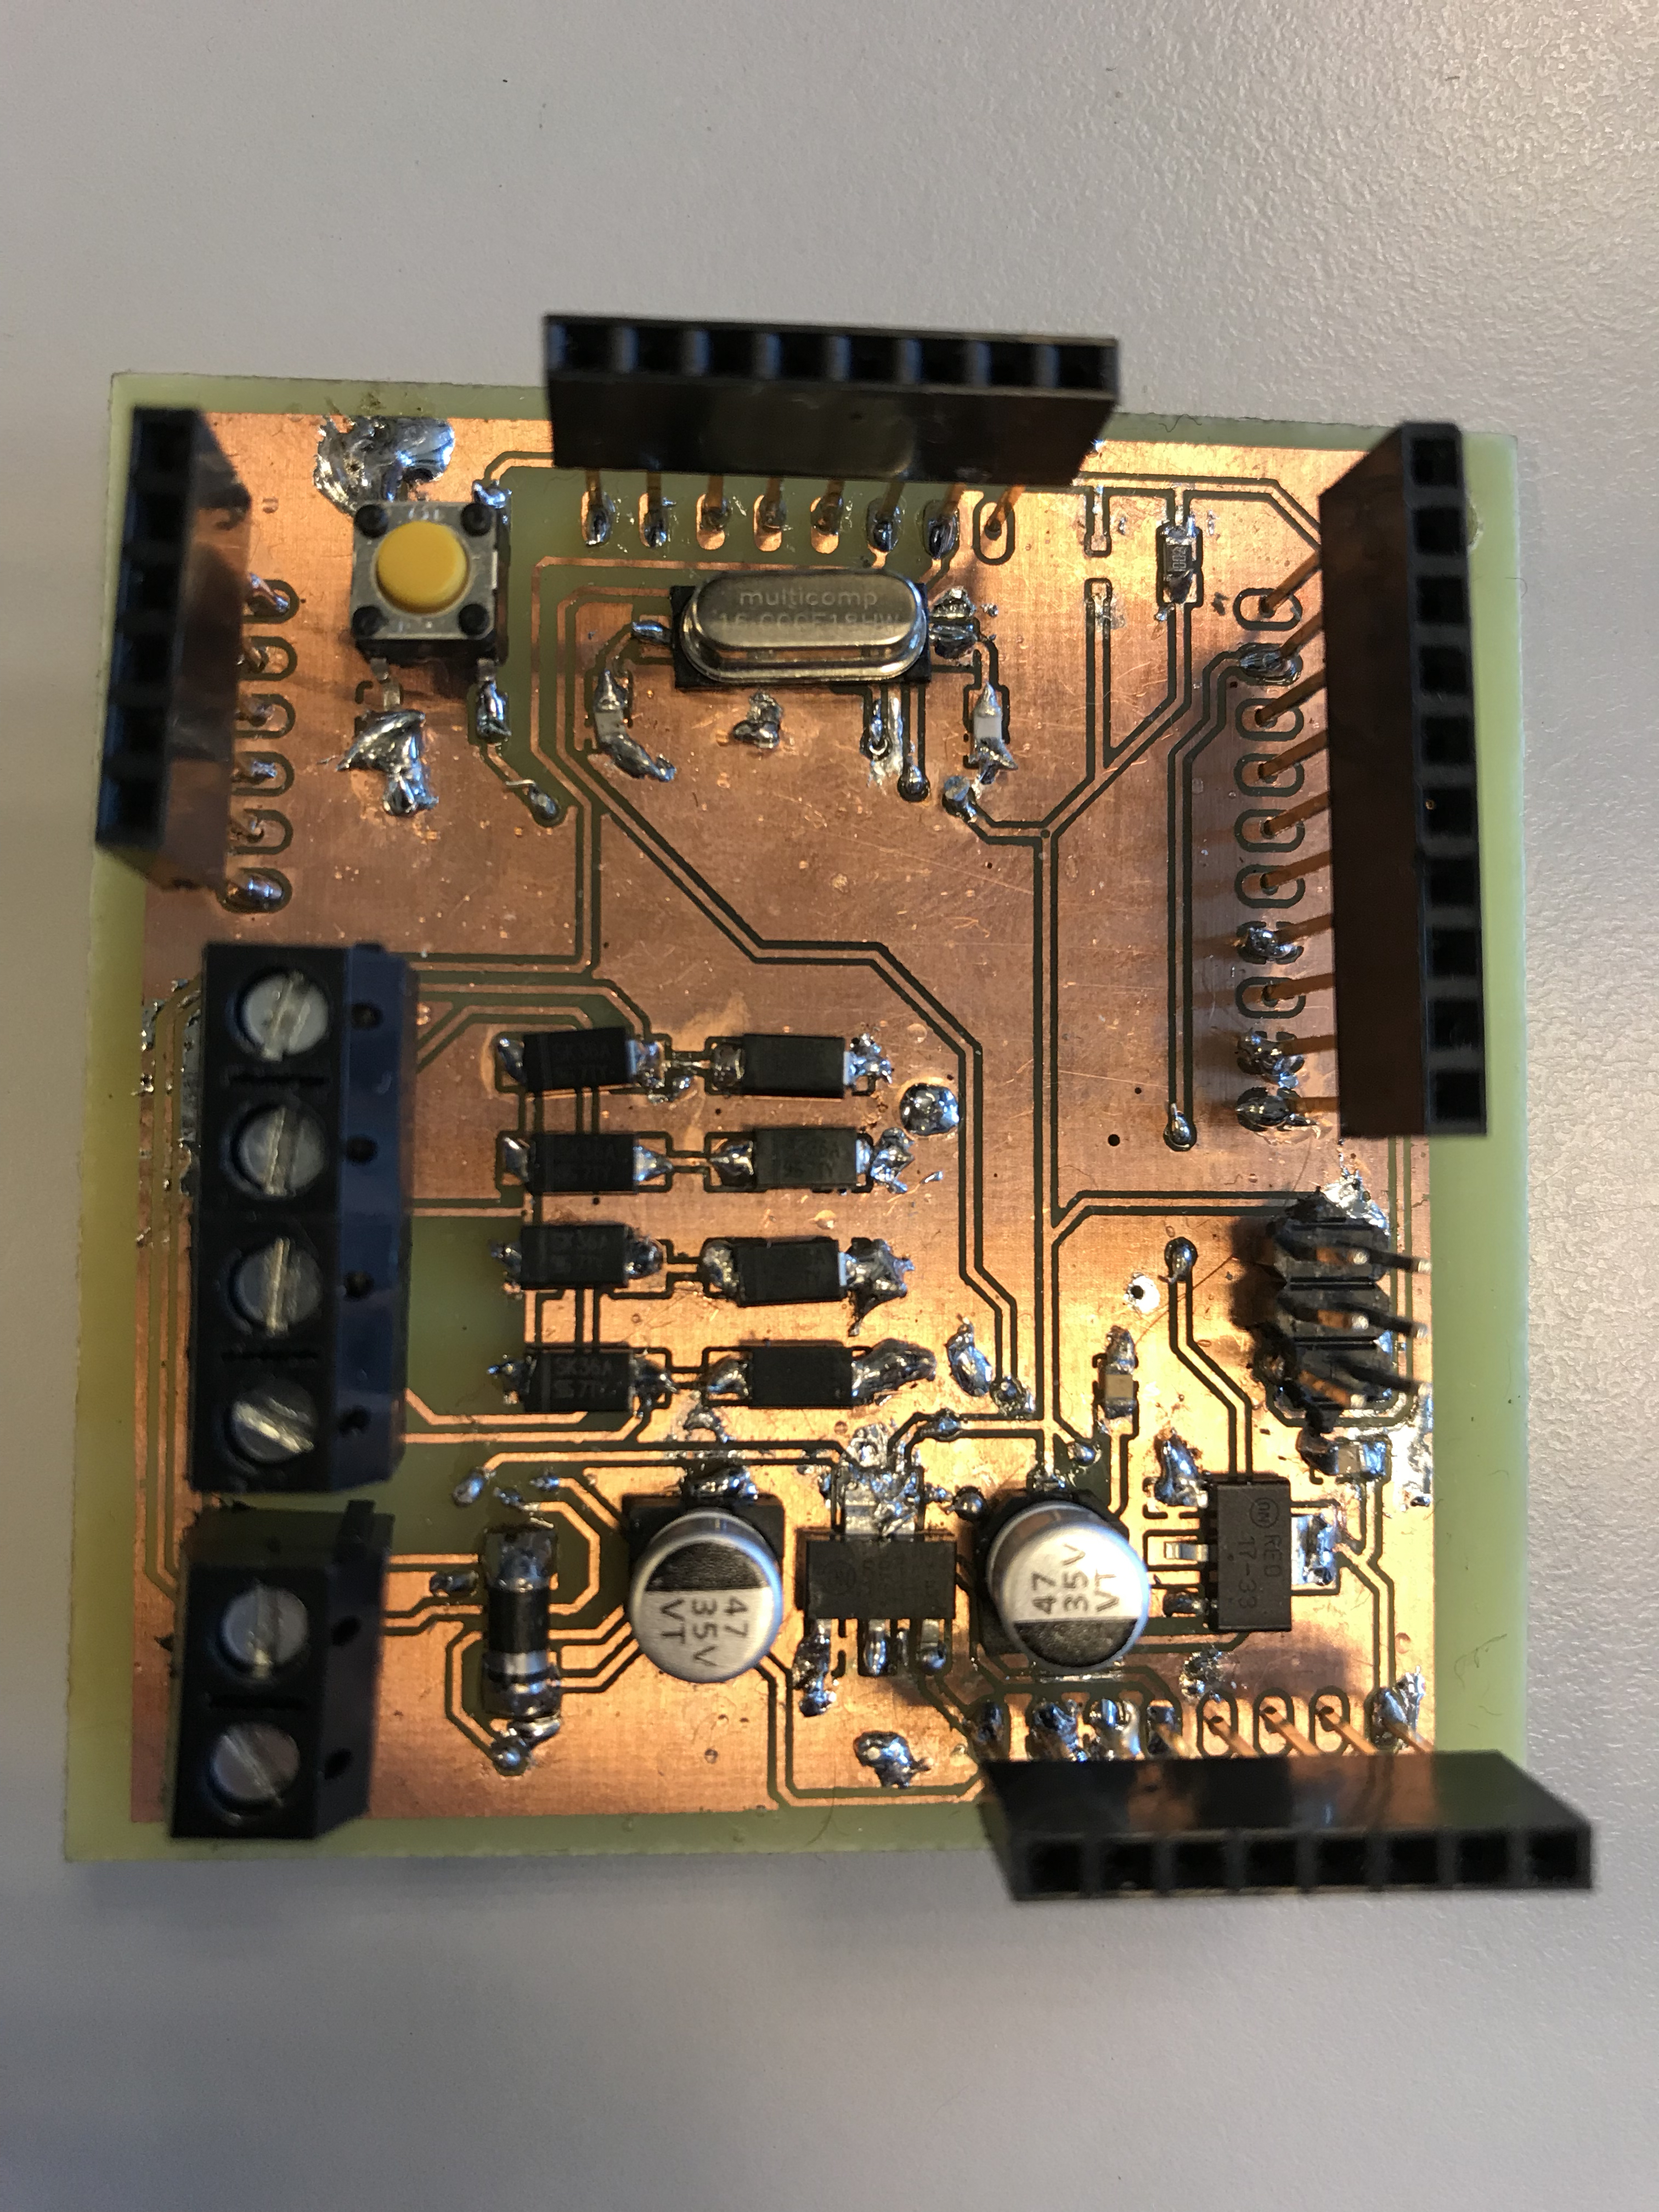
\includegraphics[width=\textwidth]{eigenpcbarduino.png}
	\caption{Bovenkant van onze custom Arduino\label{fig:custardtop}}
\end{figure}

\begin{figure}[H]
	\centering
	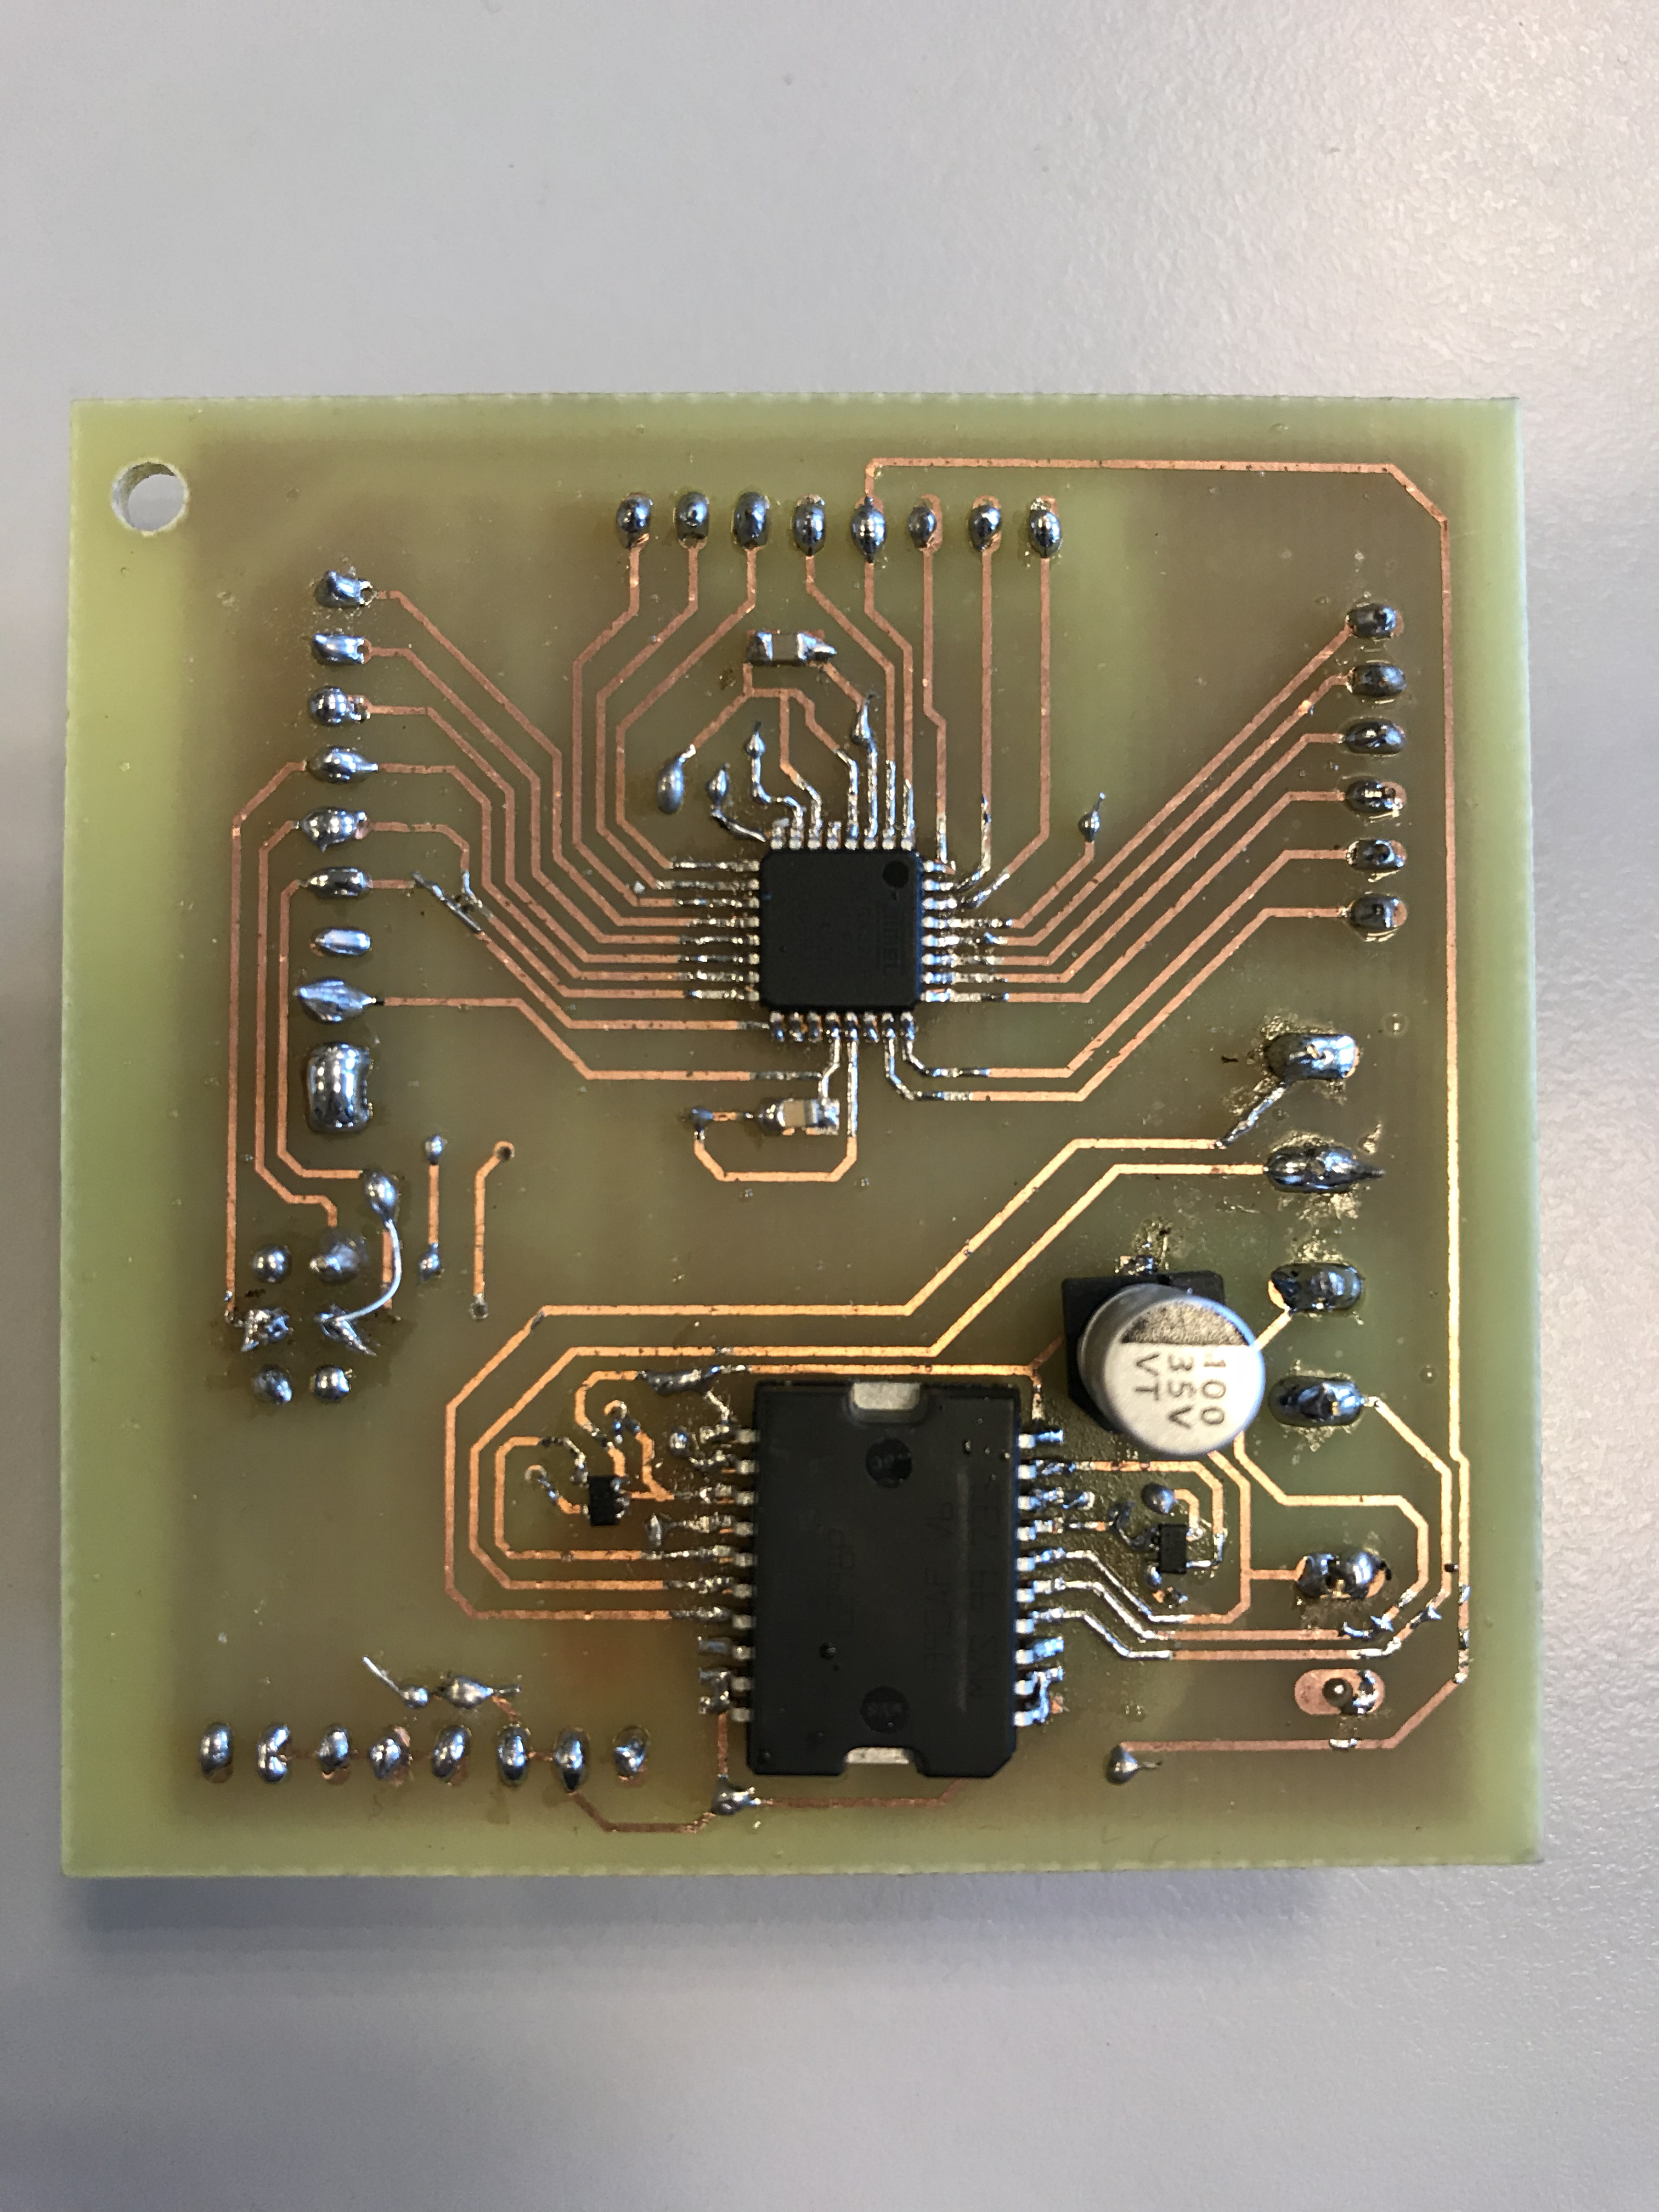
\includegraphics[width=\textwidth]{eigenpcb2.png}
	\caption{Onderkant van onze custom Arduino\label{fig:custardbot}}
\end{figure}



 
\section{Sensoren en toebehoren}
\subsection{Infrarood-sensoren}
Zoals we reeds vermeldden is het de bedoeling dat ons voertuig een parcours autonoom kan afleggen dat afgebakend wordt door twee volle witte lijnen op een zwarte ondergrond met een witte stippellijn tussen beide. Om dergelijk parcours te kunnen navigeren zullen we onderscheid moeten kunnen maken tussen de witte en zwarte ondergrond. Voor dergelijke toepassing kiezen we voor infrarood-sensoren. We zullen hiervoor gebruik maken van de TCRT-5000-sensor, zoals te zien is in figuur~\vref{fig:tcrt5000}. 

\begin{figure}[H]
	\centering
	\includegraphics[height=5cm]{tcrt5000.png}
	\caption{TCRT5000 infrarood sensor\label{fig:tcrt5000}}
\end{figure}

\subsubsection*{Sensor-cel}
De TCRT5000 bestaat uit 2 belangrijke onderdelen: ten eerste hebben we een IR-led , deze led wordt aangestuurd met een voorschakelweerstand van $330\,\mathrm{\Omega}$. Ten tweede heeft de TCRT5000 een transistor die zich in essentie als infrarood-gevoelige weerstand gedraagt, samen met een serieweerstand van $68\,\mathrm{k\Omega}$ vormt dit een spanningsdeler. De IR-led zal infraroodgolven uitstralen, naargelang de ondergrond waar dit op invalt worden deze golven quasi volledig of amper gereflecteerd. Bij een witte ondergrond zal de reflectie groot zijn en de weerstand tussen collector en emittor bijgevolg zeer klein zijn, omgekeerd hebben we bij een zwarte ondergrond een grote weerstand. De uitgangsspanning bij de spanningsdeler met de weerstand en de TCRT5000-pinnen zoals u ziet in figuur~\vref{fig:tcrt5000cel} geeft dus een maat voor de reflectieco\"effici\"ent van het oppervlak onder de sensor. De waarde van deze spanning wordt door een analoge pin ingelezen, uit deze inlezing kan dus afgeleid worden of de sensor zich boven een witte of een zwarte ondergrond bevindt. Bij een witte ondergrond bedraagt deze waarde ongeveer $30$ tot $50$ terwijl een zwarte ondergrond in een waarde tussen de $600$ en $800$ resulteert.

\begin{figure}[H]
	\centering
	\includegraphics[height=5cm]{tcrt5000cel.png}
	\caption{Sensor-cel met TCRT 5000\label{fig:tcrt5000cel}}
\end{figure}

\subsubsection*{Sensor-arrays}
Om de positie van ons voertuig te detecteren ten opzichte van een witte zijlijn maakten we twee sensor-arrays van elk vier sensoren die via een multiplexer op een aparte printplaat ingelezen worden in \'e\'en analoge pin. We positioneerden deze linksvooraan en linksachteraan het wagentje met behulp van 3D-geprinte en verstelbare armen, op deze manier kunnen we de zijlijn langs de linkerkant van het parcours detecteren. Het voordeel hiervan is ook dat we in de bochten van de baan vrij stabiel kunnen bijsturen. Na een aantal verschillende positioneringen bleek dit de beste resultaten op te leveren. De positionering van de sensor-arrays is te zien in figuur~\vref{fig:sensorarraypositionering}. In figuren~\vref{fig:sensorarrayvooraan} en~\vref{fig:sensorarrayachteraan} ziet u de twee verschillende sensorarrays aan de onderzijde.

\begin{figure}[H]
	\centering
	\includegraphics[height=5cm]{sensorarraypositionering.png}
	\caption{Sensorarray op het wagentje ten opzichte van de zijlijn\label{fig:sensorarraypositionering}}
\end{figure}

\begin{figure}[H]
	\centering
	\begin{minipage}[b]{0.4\textwidth}
		\centering
		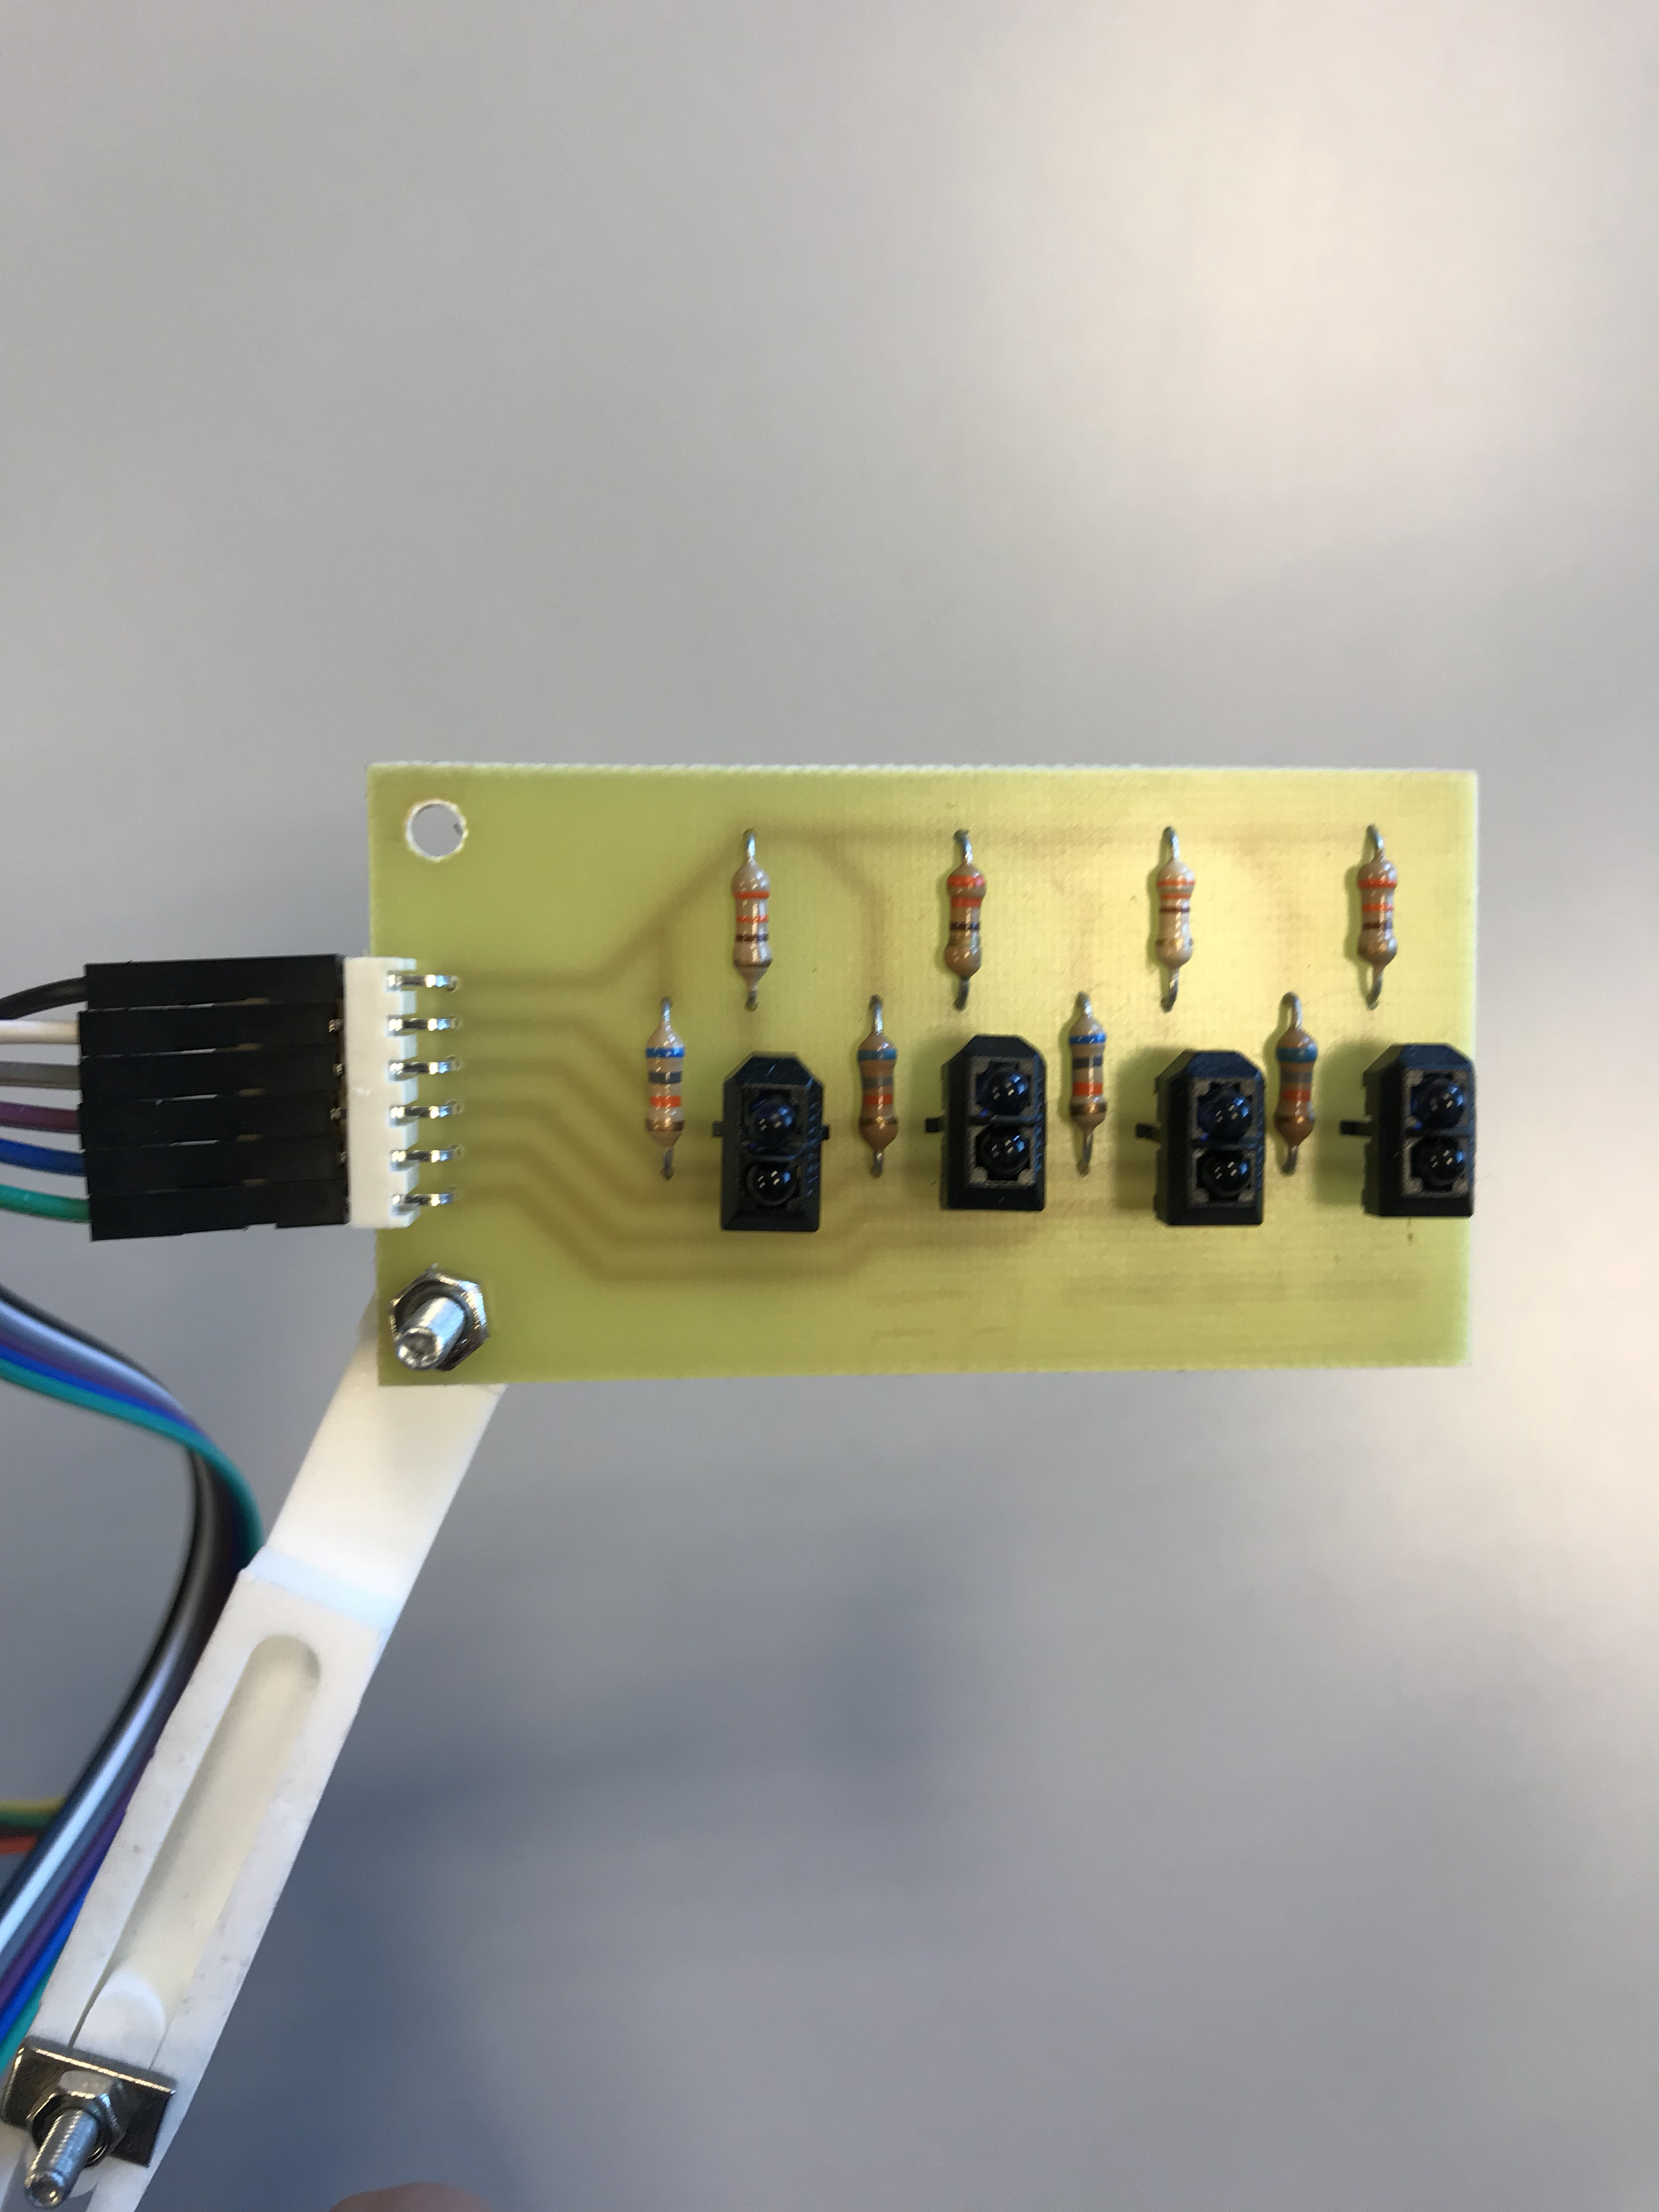
\includegraphics[height=5cm]{sensorarrayvooraanonderkant.png}
		\caption{Sensorarray linksvooraan}
		\label{fig:sensorarrayvooraan}
	\end{minipage}
	\hfill
	\begin{minipage}[b]{0.4\textwidth}
		\centering
		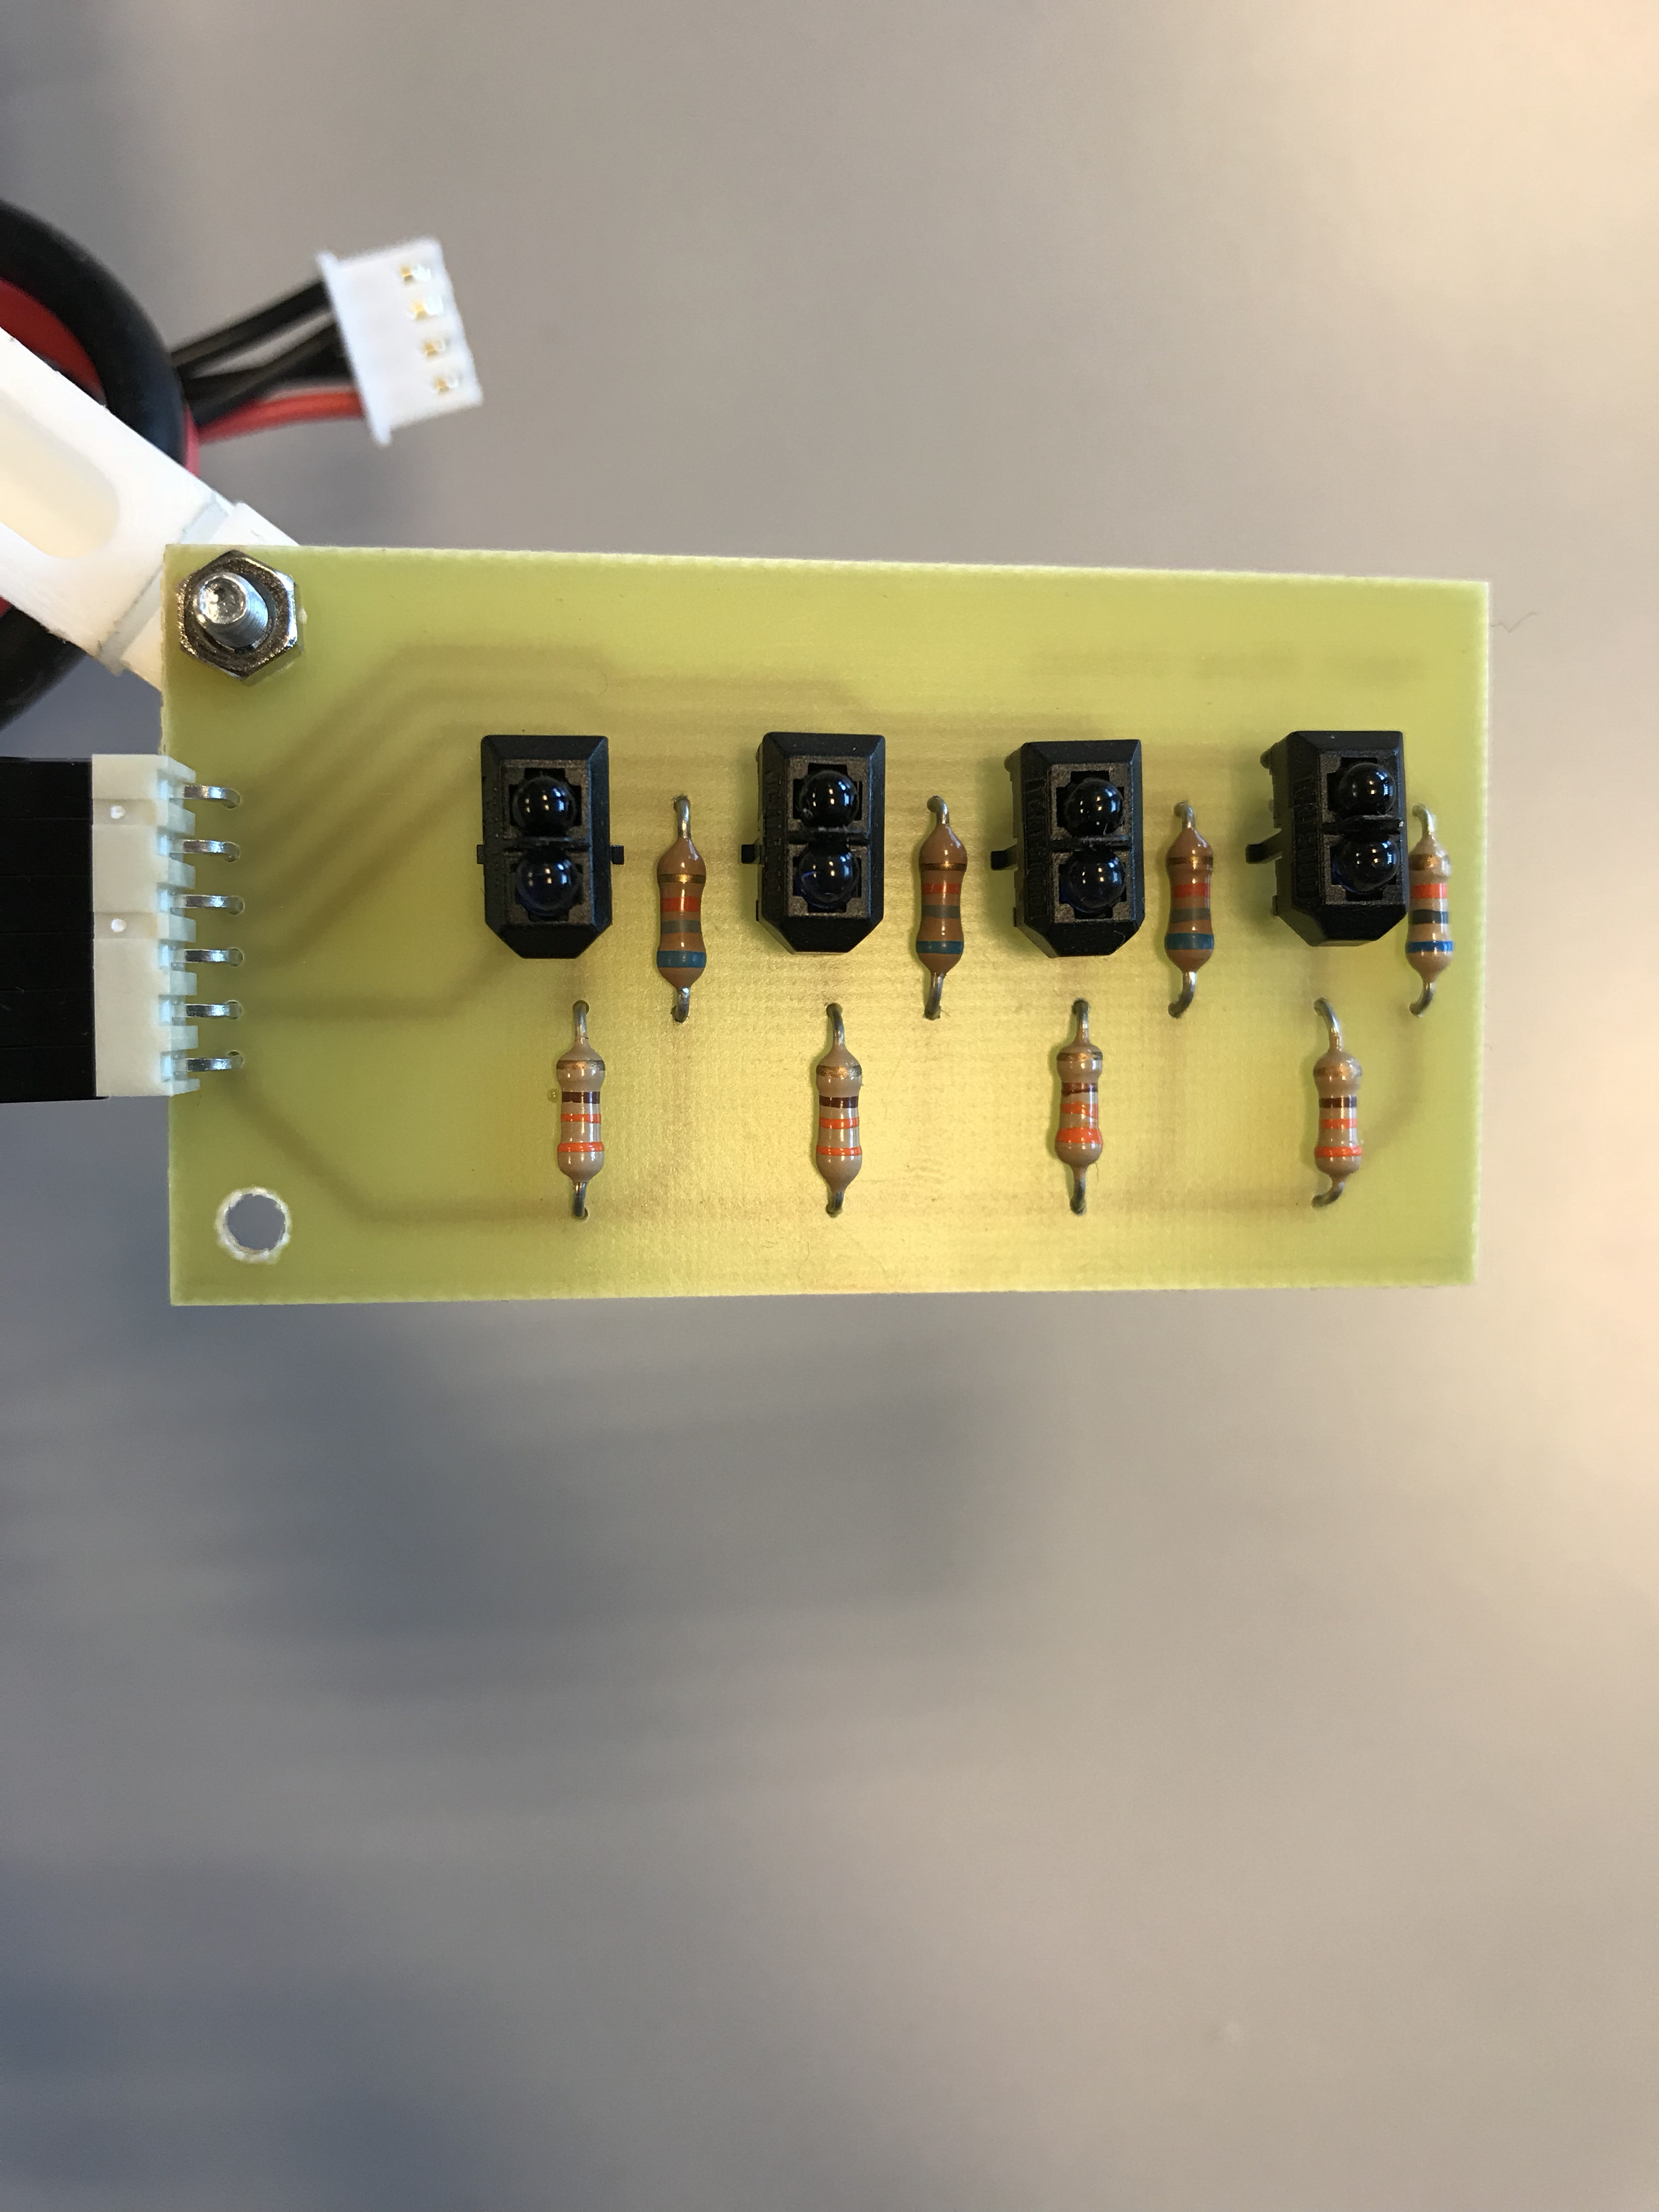
\includegraphics[height=5cm]{sensorarrayachteraanonderkant.png}
		\caption{Sensorarray linksachteraan}
		\label{fig:sensorarrayachteraan}
	\end{minipage}
\end{figure}

\subsection{Multiplexers}
Aangezien we slechts over een beperkt aantal analoge ingangen beschikken zullen we de verschillende sensoren moeten multiplexen, hiervoor maken we gebruik van een CD4051BE-multiplexer op een aparte PCB vooraan het wagentje. In figuur~\vref{fig:cd4051be_pinout} ziet u de pin-out van dit IC, de PCB met de multiplexer is te zien in figuur~\vref{fig:muxvooraan}. We gebruiken deze multiplexer om de acht sensoren in de twee sensor-arrays in te kunnen lezen op \'e\'en analoge pin: A0. We gebruiken hiervoor drie digitale pinnen D0,D1 en D2, die de bit selects van de multiplexer aansturen.

\begin{figure}[H]
	\centering
	\begin{minipage}[b]{0.4\textwidth}
		\includegraphics[height=5cm]{cd4051be_pinout.png}
		\caption{CD4051BE multiplexer pin-out}
		\label{fig:cd4051be_pinout}
	\end{minipage}
	\hfill
	\begin{minipage}[b]{0.4\textwidth}
		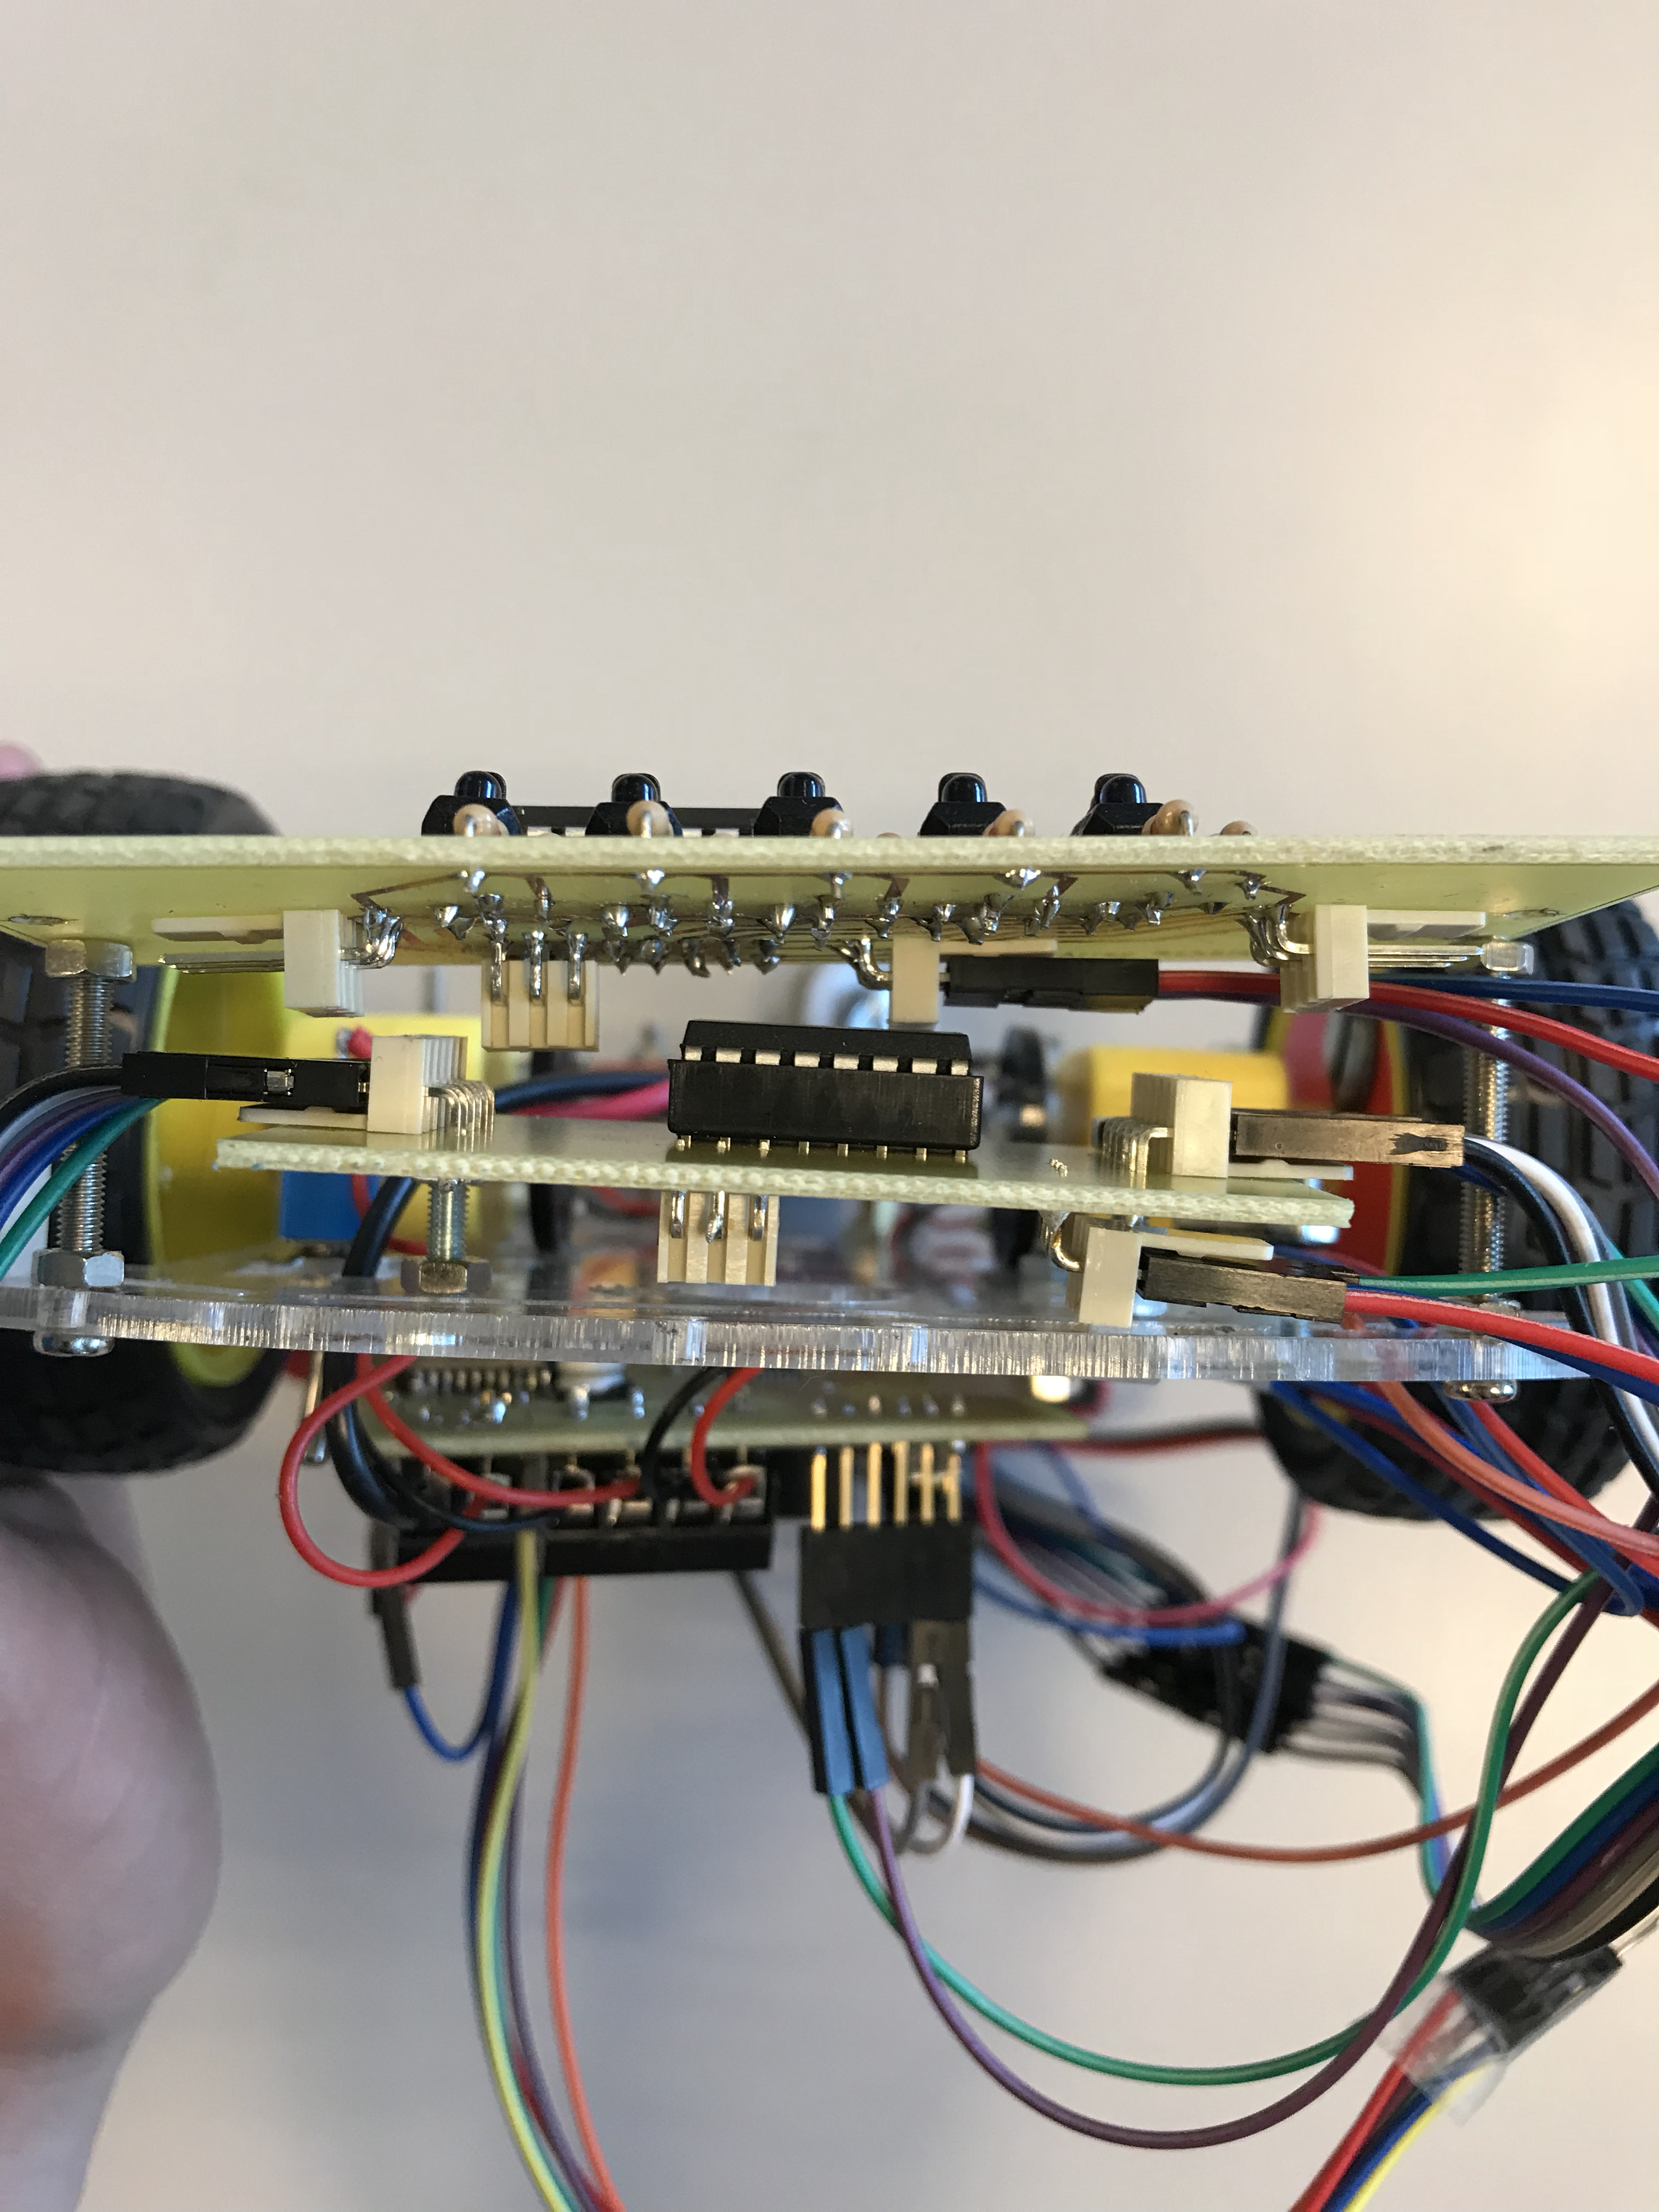
\includegraphics[height=5cm]{muxvooraan.png}
		\caption{PCB met CD4051BE multiplexer vooraan het wagentje}
		\label{fig:muxvooraan}
	\end{minipage}
\end{figure}
\subsection{Hall-sensor en magneten}\label{sec:hall-sensor}
Voor het meten van de snelheid zullen we moeten bepalen hoeveel rotaties de wielen maken gedurende een bepaalde periode. Uit dit aantal rotaties kunnen we vervolgens de afgelegde weg en dus ook de snelheid berekenen. We hebben dus een manier nodig om te detecteren wanneer en hoeveel keer het wiel een rotatie maakt, daarvoor kozen we voor het gebruik van een Hall-sensor die het passeren van magneten gemonteerd in de wielas detecteert. De gebruikte Hall-sensor is de SS41 digitale Hall-sensor van Honeywell die gevoed wordt op $5\,\mathrm{V}$. De output van deze sensor wordt aangesloten aan pin D4. In figuur ~\vref{fig:wielmagneten} ziet u de magneten die binnen in de wielas gemonteerd werden, merk op dat deze magneten een tegengestelde polarisatie hebben zodanig dat de output van de Hall-sensor correct omschakelt als deze magneten beurtelings passeren. In figuur~\vref{fig:hallsensor} ziet u hoe de Hall-sensor bij het wiel gemonteerd is.

\begin{figure}[H]
	\centering
	\begin{minipage}[b]{0.4\textwidth}
		\centering
		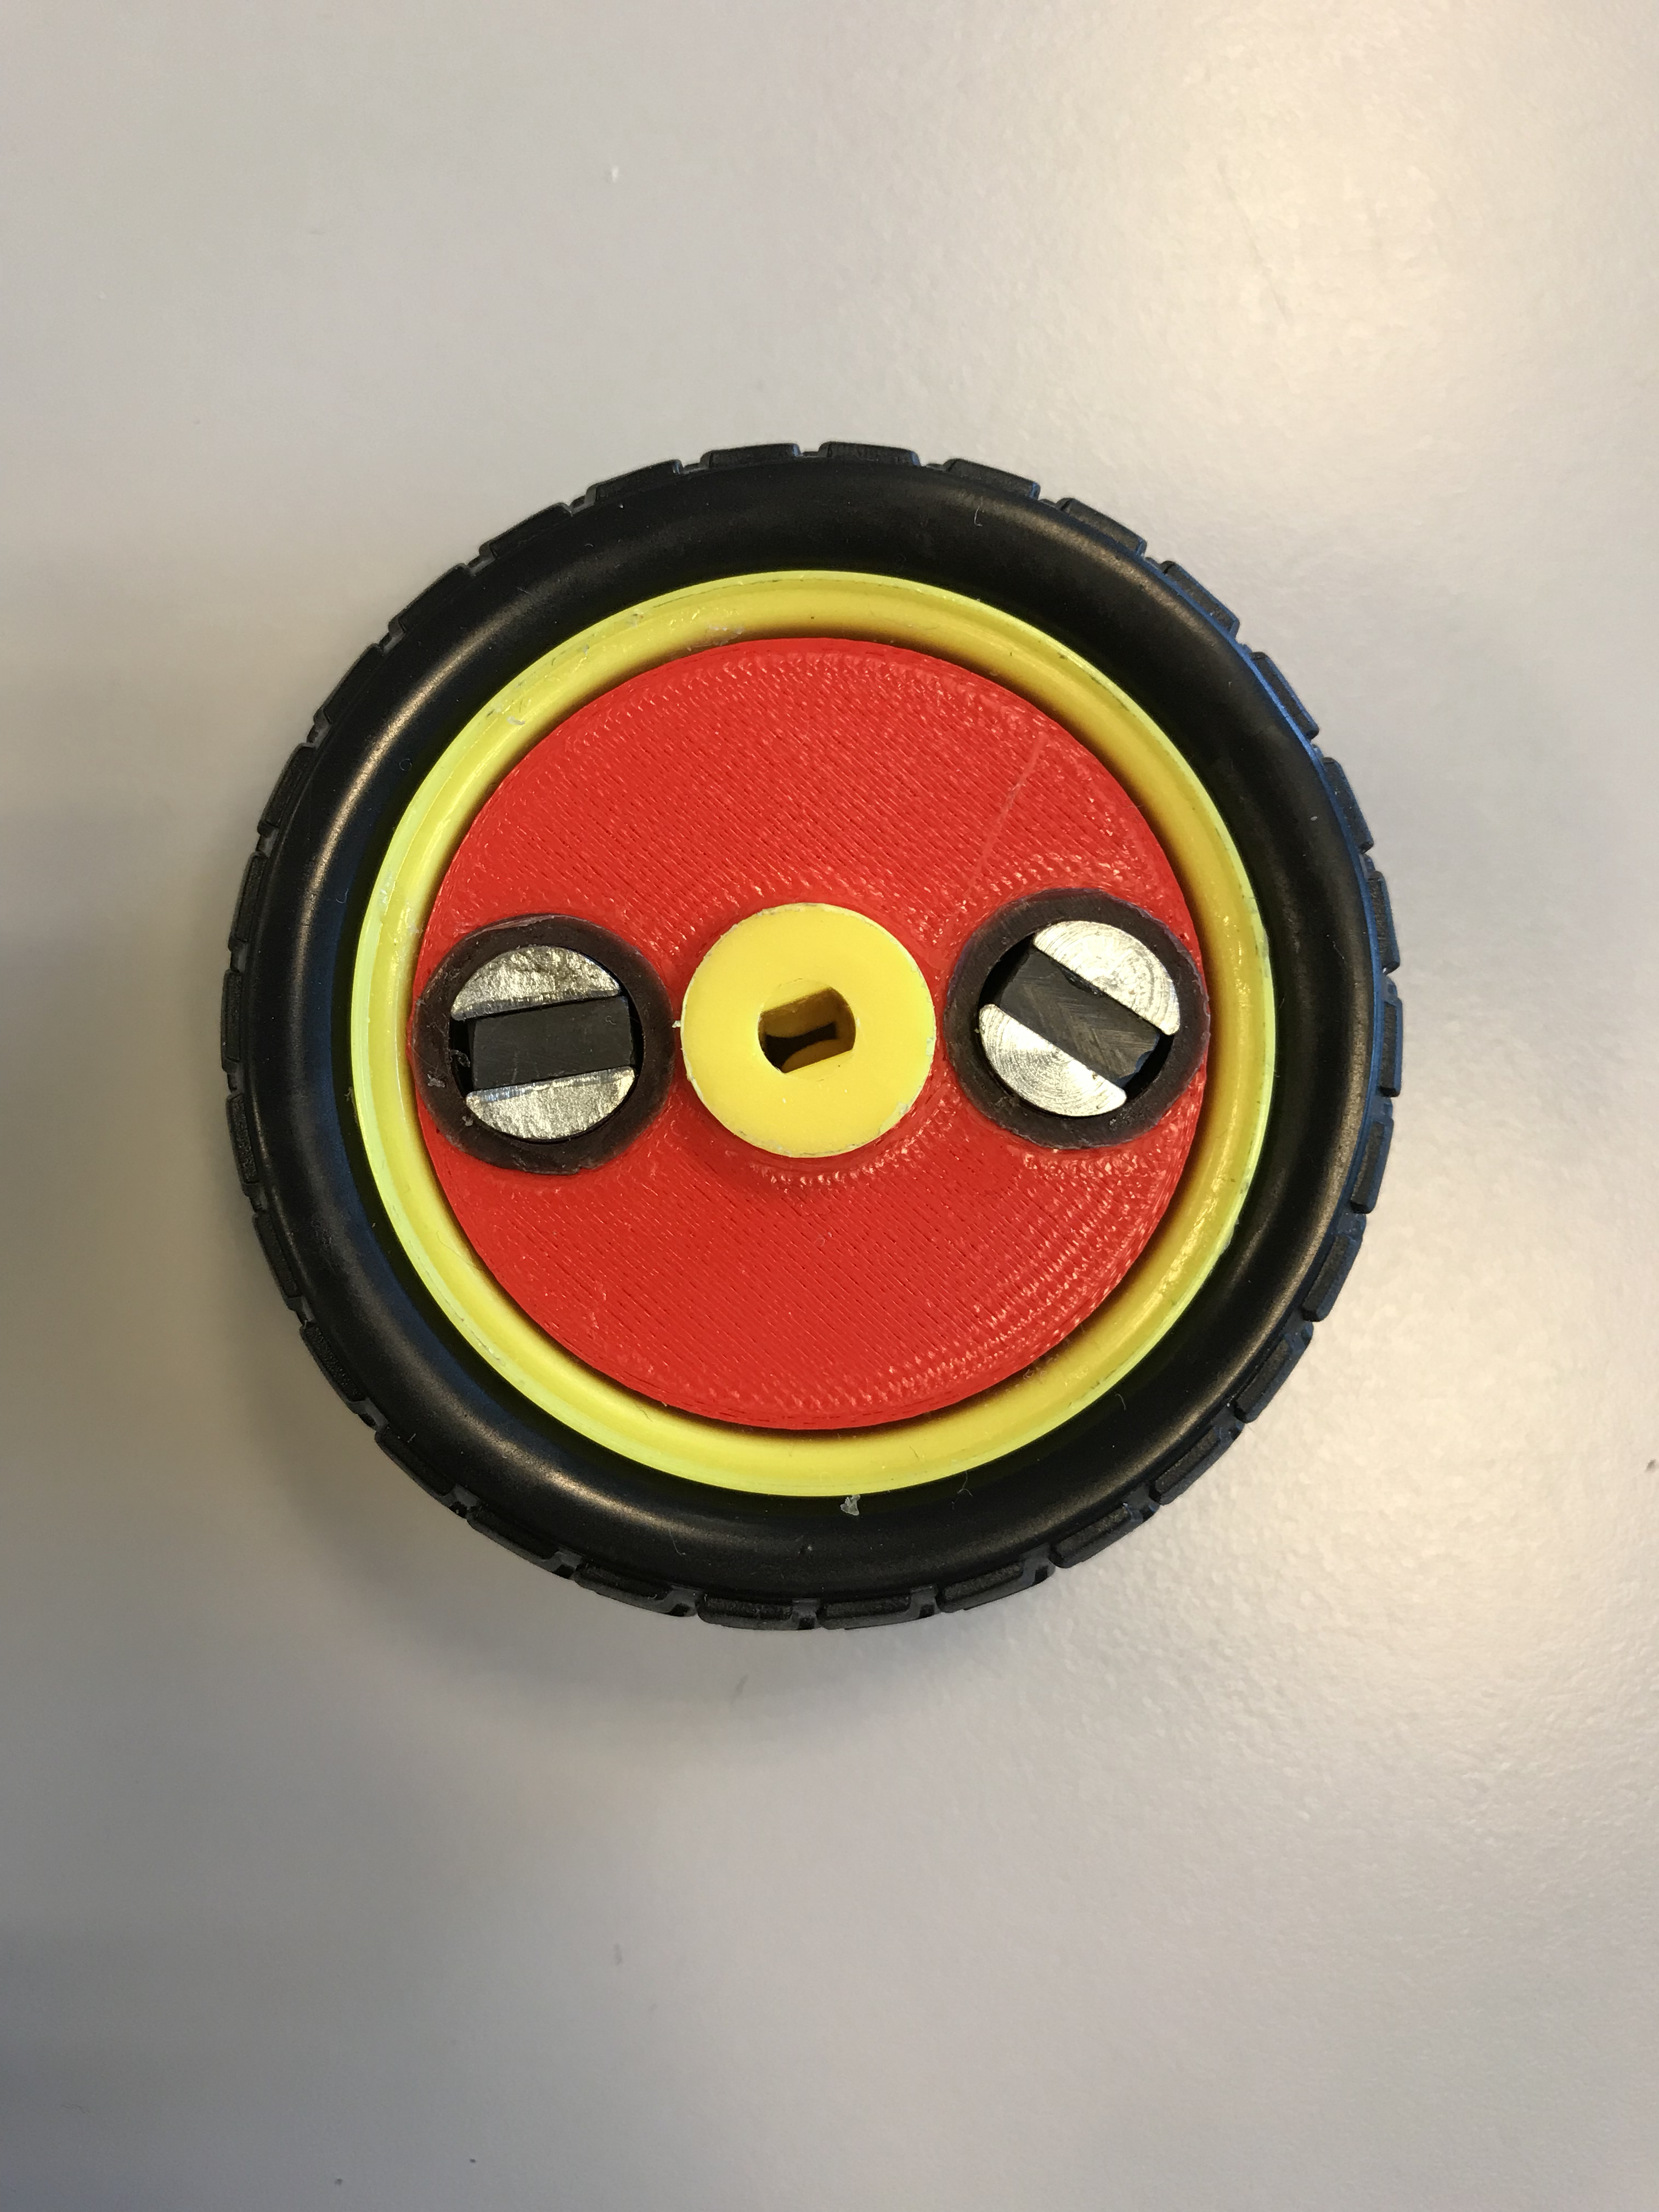
\includegraphics[height=5cm]{wielmagneten.png}
		\caption{Magneten gemonteerd in wielas\label{fig:wielmagneten}}
	\end{minipage}
	\hfill
	\begin{minipage}[b]{0.4\textwidth}
		\centering
		\includegraphics[height=5cm]{hallsensor.png}
		\caption{Hall-sensor gemonteerd naast wiel\label{fig:hallsensor}}
	\end{minipage}
\end{figure}

\subsection{RFID-reader}
Het inlezen van de RFID-tags gebeurt met behulp van de PN532 NFC-module v3 van Elechouse die u ziet in figuren~\ref{fig:pn532} en~\ref{fig:rfidlezermontage}. Deze module is voorzien van aansluitingen voor communicatie over HSU (High Speed UART), I\textsuperscript{2}C en SPI. De gewenste communicatie-interface wordt gekozen aan de hand van de twee SMD-switches op de module. We maken gebruik van I\textsuperscript{2}C om de tags in te lezen, de reden van deze keuze zullen we verder bespreken in hoofdstuk~\vref{sec:problemen-en-moeilijkheden}. We sluiten dus volgende pinnen van de PN532-module aan:
\begin{itemize}
	\item GND: Ground van de module, aangesloten aan de GND van onze Arduino.
	\item VCC: Voeding van de module, aangesloten aan 5\,V van onze Arduino.
	\item SDA: Seri\"ele data-pin van de module, wordt aangesloten aan pin A4 van onze Arduino.
	\item SDA: Seri\"ele clock-pin van de module, wordt aangesloten aan pin A5 van onze Arduino.
\end{itemize}

\begin{figure}[H]
	\centering
	\begin{minipage}[b]{0.4\textwidth}
		\centering
		\includegraphics[height=5cm]{rfidlezer.png}
		\caption{PN532 NFC-module\label{fig:pn532}}
	\end{minipage}
	\hfill
	\begin{minipage}[b]{0.4\textwidth}
		\centering
		\includegraphics[height=5cm]{rfidlezermontage.png}
		\caption{PN532 op het wagentje\label{fig:rfidlezermontage}}
	\end{minipage}
\end{figure}
\subsection{Bluetooth-module}
Een onderdeel van de opdracht bestond er uit om communicatie te voorzien tussen ons wagentje met een Arduino-microcontroller enerzijds, en een Raspberry Pi anderzijds. Om dit te realiseren kozen we er voor om Bluetooth te gebruiken.
We maken gebruik van een HC05 Bluetooth-module om deze communicatie mogelijk te maken.
Deze module ziet u in figuren~\ref{fig:hc05} en~\ref{fig:hc05montage}. De HC05 beschikt over zes pinnen:
\begin{itemize}
	\item EN: Dit is een enable voor de module die actief laag is, deze moet niet aangesloten worden aangezien we de module constant actief willen.
	\item VCC: Voeding van de module, aangesloten aan 5\,V van onze Arduino.
	\item GND: Ground van de module, aangesloten aan de GND van onze Arduino.
	\item TXD: Transmit-pin van de module, aangesloten aan RX van de Arduino op pin D7
	\item RXD: Receive-pin van de module, aangesloten aan TX van de Arduino op pin D8
	\item STATE: Geeft informatie over de toestand van de module, gaat hoog wanneer deze verbonden is en laag wanneer dat niet het geval is. Deze pin wordt niet gebruikt voor onze toepassing
\end{itemize}

\begin{figure}[H]
	\centering
	\begin{minipage}[b]{0.4\textwidth}
		\centering
		\includegraphics[height=5cm]{hc05.png}
		\caption{HC05 Bluetooth-module\label{fig:hc05}}
	\end{minipage}
	\hfill
	\begin{minipage}[b]{0.4\textwidth}
		\centering
		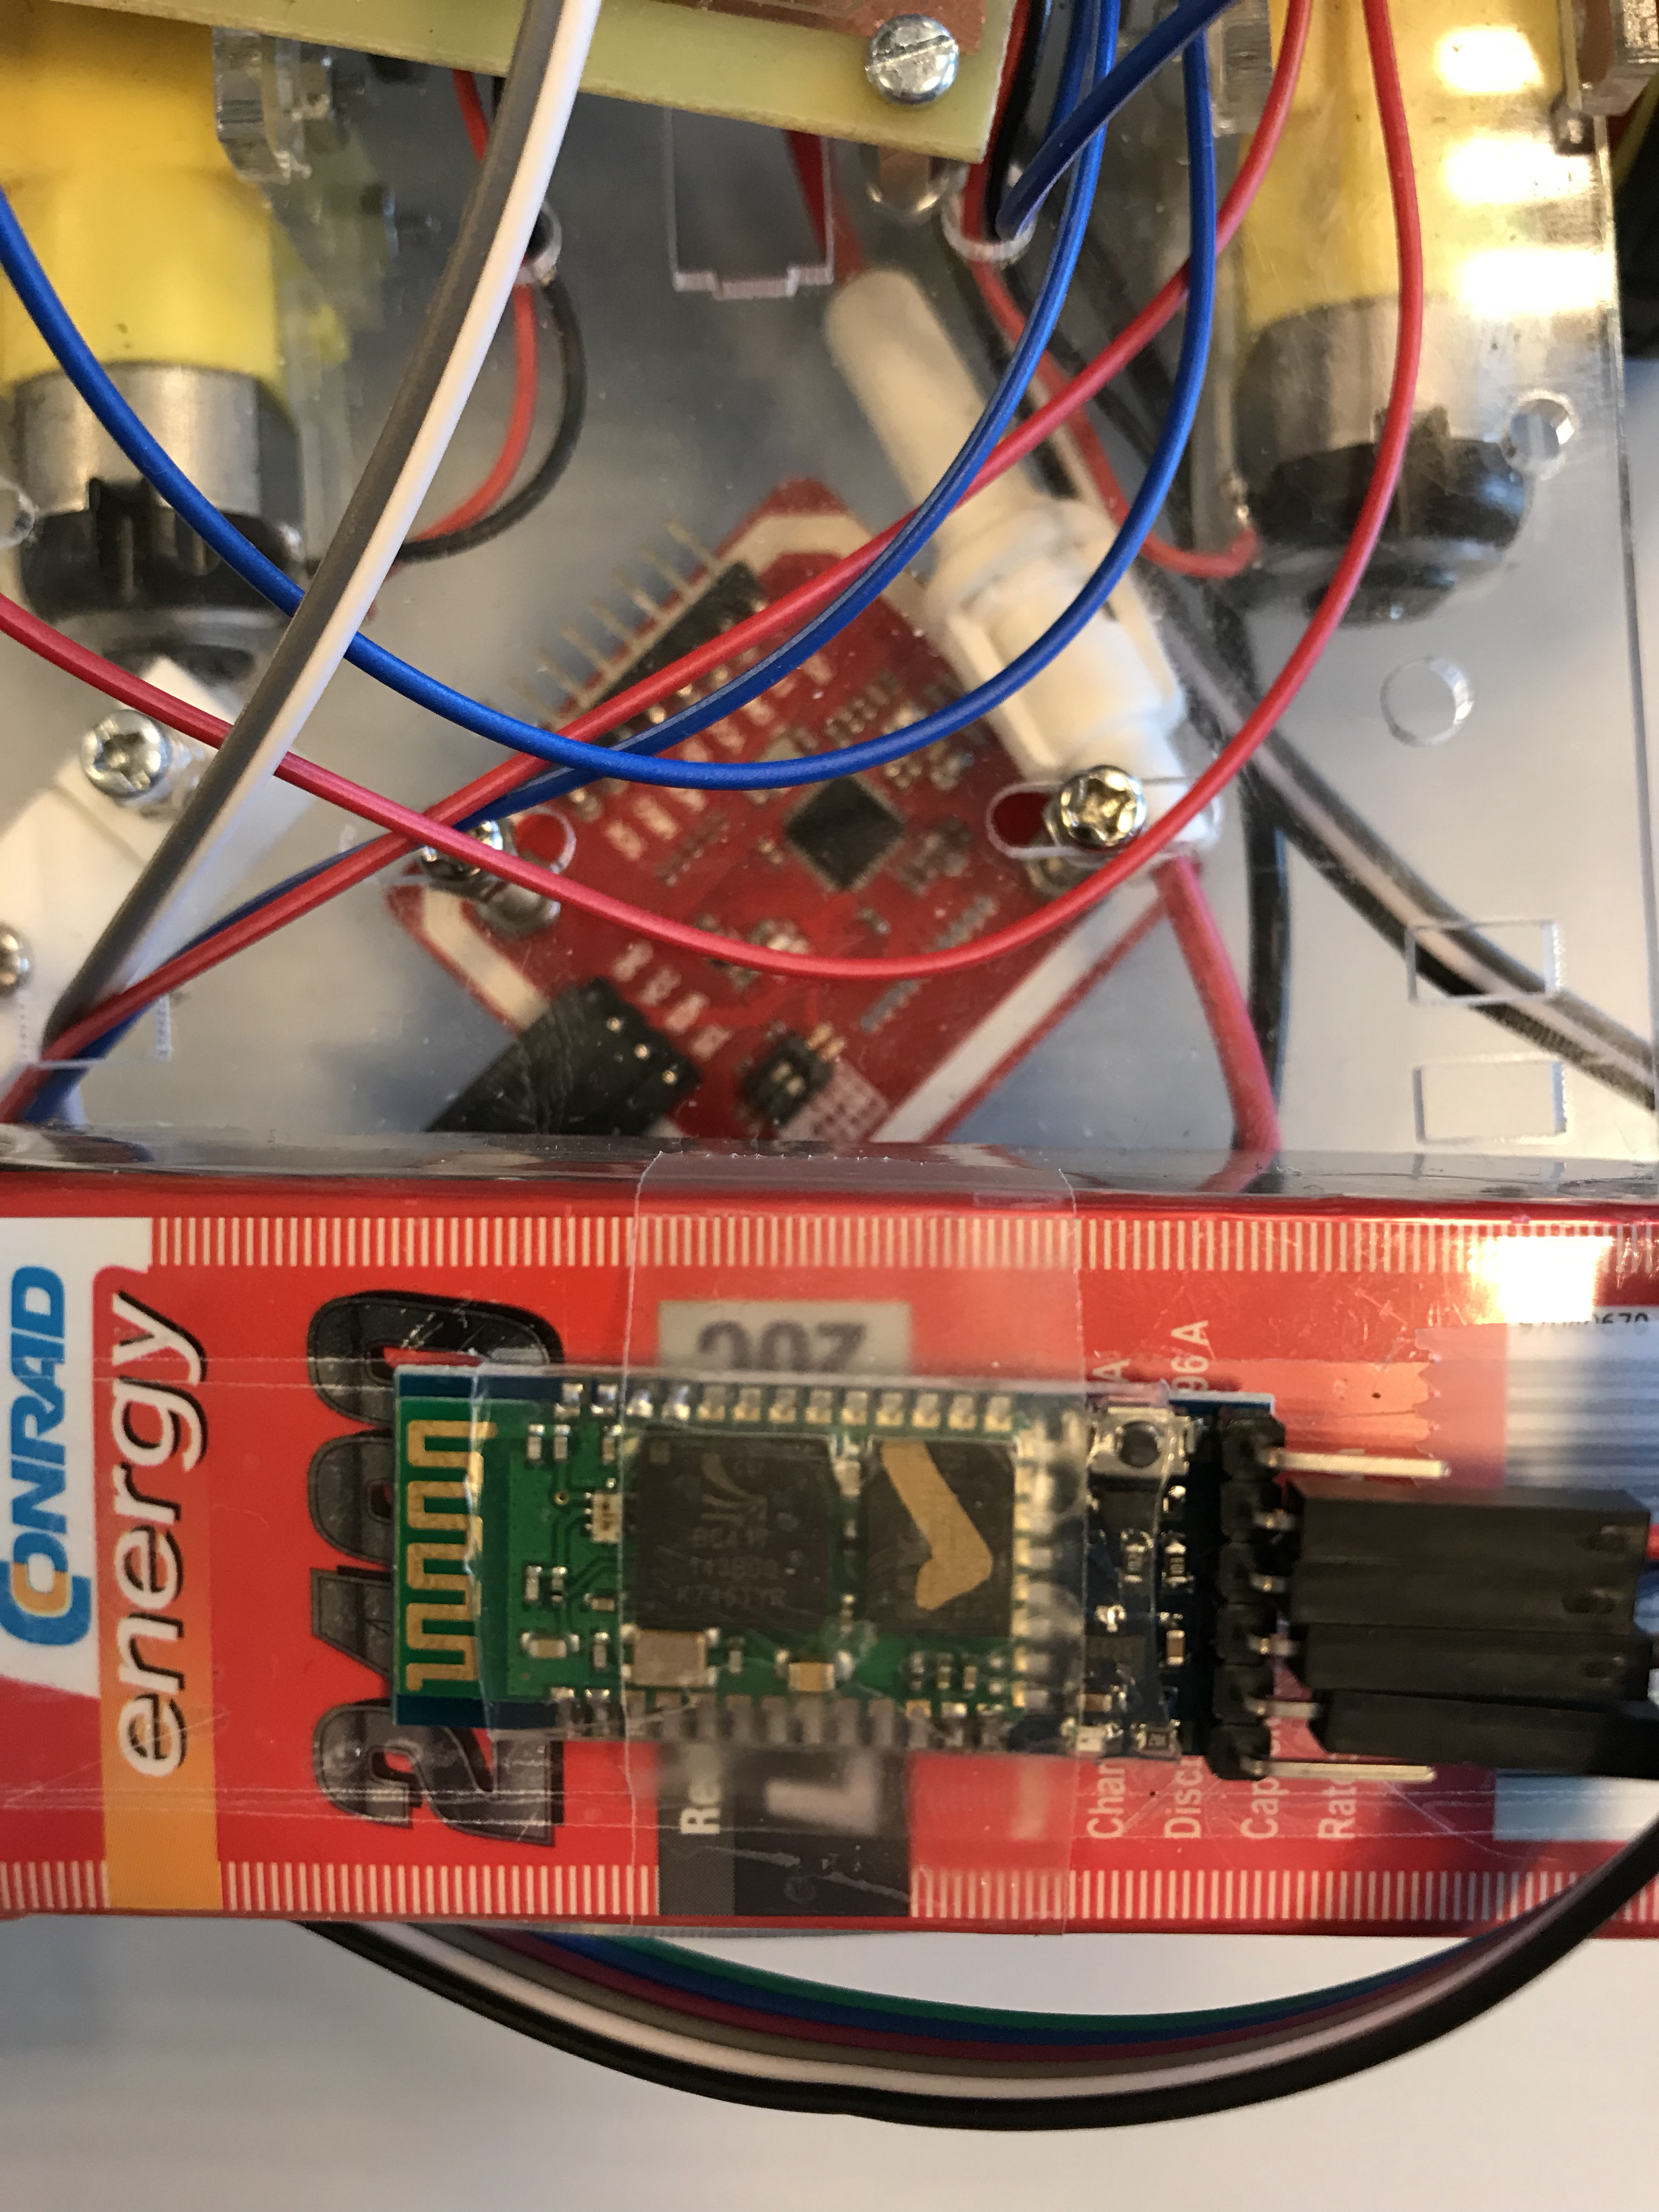
\includegraphics[height=5cm]{bluetoothenrfidlezer.png}
		\caption{HC05 Bluetooth-module op het wagentje\label{fig:hc05montage}}
	\end{minipage}
\end{figure}

\subsection{Pintoewijzing}
We zagen in voorgaande secties het ontwerp van ons custom Arduino board en de bijkomende hardware. In tabel~\ref{table:pintoewijzing} ziet u een overzicht van de aansluitingen tussen deze hardware en de pinnen van het board.

\begin{table}[H]
	\setlength\aboverulesep{0pt}
	\setlength\belowrulesep{0pt}
	\centering
	\resizebox{\textwidth}{!}{%
		\begin{tabular}{@{}|l|l|l|l|l|l|@{}}
			\toprule
			Pin         & Input/Output & Aansluiting       & Pin          & Input/Output & Aansluiting    \\ \midrule
			D0          & OUT          & MUX Bit select 2  & D10 ($\sim$) & /            & /              \\ \midrule
			D1          & OUT          & MUX Bit select 1  & D11 ($\sim$) & /            & /              \\ \midrule
			D2          & OUT          & MUX Bit select 0  & D12          & /            & /              \\ \midrule
			D3 ($\sim$) & OUT          & PWM Motor A       & D13          & /            & /              \\ \midrule
			D4          & IN           & Hall Sensor Input & A0           & IN            & IR-sensoren    \\ \midrule
			D5 ($\sim$) & OUT          & Richting Motor A  & A1           & /            & /              \\ \midrule
			D6 ($\sim$) & OUT          & Richting Motor B  & A2           & /            & /              \\ \midrule
			D7          & IN           & Bluetooth RX      & A3           & /            & /              \\ \midrule
			D8          & OUT          & Bluetooth TX      & A4           & IN            & RFID-lezer SDA \\ \midrule
			D9 ($\sim$) & OUT          & PWM Motor B       & A5           & OUT            & RFID-lezer SCL \\ \bottomrule
		\end{tabular}%
	}
	\caption{Pintoewijzing van custom Arduino}
	\label{table:pintoewijzing}
\end{table}

\section{Raspberry Pi}
Ten slotte hebben we nog de Raspberry Pi. We maken gebruik van een Raspberry Pi 3 zoals u ziet in figuur~\vref{fig:rpi3}. Dit is in principe een computer waarop een Linux-distributie draait. We sluiten op de RPi3 via USB nog een muis en toetsenbord aan, de monitor wordt verbonden met een HDMI-kabel. We maken geen gebruik van de voorziene I/O-pinnen. Belangrijk is dat deze Raspberry Pi 3 een ingebouwde Bluetooth-adapter heeft en we dus geen bijkomende Bluetooth-dongle nodig hebben. 
\begin{figure}[H]
	\centering
	\includegraphics[height=5cm]{rpi3.png}
	\caption{Raspberry Pi 3\label{fig:rpi3}}
\end{figure}
\chapter{Toelichting software}\label{sec:toelichting-software}
\section{IR-sensoren inlezen}
Voor het inlezen van de sensoren wordt gebruik gemaakt van \'e\'en analoge pin, met deze pin lezen we de waardes van alle acht sensoren in via een multiplexer. Deze multiplexer wordt aangestuurd aan de hand van drie digitale pinnen die dienst doen als bit select. Om de tijdsduur voor het inlezen van de infrarood-sensoren via de multiplexer te minimaliseren lezen we deze in aan de hand van Gray-code. De volgorde van inlezen wordt verduidelijkt in tabel~\vref{table:graycode}. De ingelezen waarden worden opgeslagen in een array van acht integers. De waardes in de array worden vervolgens gedigitaliseerd aan de hand van een grenswaarde, hiervoor hebben we de waarde $300$ gekozen. Indien de sensorwaarde onder deze grens ligt ziet de sensor een witte ondergrond en krijgt dit digitaal een waarde '$1$', als de waarde boven de grens ligt komt dit overeen met een zwarte ondergrond en een digitale waarde '$0$'. 

\begin{table}[H]
	\centering
	\begin{tabular}{|l|l|l|l|l|l|}
		\hline
		\# & Bit Select 2 & Bit Select 1 & Bit Select 0 & MUX-pin & Sensor      \\ \hline
		0  & 0            & 0            & 0            & 13      & Vooraan 2   \\ \hline
		1  & 0            & 0            & 1            & 14      & Vooraan 3   \\ \hline
		3  & 0            & 1            & 1            & 12      & Vooraan 1   \\ \hline
		2  & 0            & 1            & 0            & 15      & Vooraan 4   \\ \hline
		6  & 1            & 1            & 0            & 2       & Achteraan 3 \\ \hline
		7  & 1            & 1            & 1            & 7       & Achteraan 2 \\ \hline
		5  & 1            & 0            & 1            & 5       & Achteraan 1 \\ \hline
		4  & 1            & 0            & 0            & 7       & Achteraan 1 \\ \hline
	\end{tabular}
	\caption{Inlezen van sensoren aan de hand van Grey-code}
	\label{table:graycode}
\end{table}

\section{Rijden en PID-regeling}
Nu de sensoren ingelezen kunnen worden is het mogelijk om aan de hand hiervan de positie van het wagentje ten opzichte van de zijlijn te bepalen.
Hiermee kan vervolgens het wagentje correct bijgestuurd worden om deze lijn te volgen. Om dit te realiseren wordt PID-regeling toegepast.
Deze PID-regeling gebeurt aan de hand van een foutwaarde die afgeleid wordt uit de ingelezen sensorwaarden, aan elke sensor wordt dus een gewicht toegekend die een maat geeft voor de afwijking ten opzichte van de witte lijn. Deze gewichten vindt u in tabel~\vref{table:sensorgewicht}.

\begin{table}[H]
	\centering
	\begin{tabular}{lllll}
		\hline
		\multicolumn{1}{|l|}{}           & \multicolumn{1}{l|}{Vooraan 1}   & \multicolumn{1}{l|}{Vooraan 2}   & \multicolumn{1}{l|}{Vooraan 3}   & \multicolumn{1}{l|}{Vooraan 4}   \\ \hline
		\multicolumn{1}{|l|}{Foutwaarde} & \multicolumn{1}{l|}{-3}          & \multicolumn{1}{l|}{-1}          & \multicolumn{1}{l|}{1}           & \multicolumn{1}{l|}{3}           \\ \hline
		&                                  &                                  &                                  &                                  \\ \hline
		\multicolumn{1}{|l|}{}           & \multicolumn{1}{l|}{Achteraan 1} & \multicolumn{1}{l|}{Achteraan 2} & \multicolumn{1}{l|}{Achteraan 3} & \multicolumn{1}{l|}{Achteraan 4} \\ \hline
		\multicolumn{1}{|l|}{Foutwaarde} & \multicolumn{1}{l|}{3}           & \multicolumn{1}{l|}{1}           & \multicolumn{1}{l|}{-1}          & \multicolumn{1}{l|}{-3}           \\ \hline
	\end{tabular}
	\caption{Gewichten van sensoren}
	\label{table:sensorgewicht}
\end{table}

De foutwaarde van de voorste sensoren wordt nu berekend met volgende formule:
\begin{gather*}
E_{vooraan} = \frac{\sum\limits_{i=1}^{4}S_{vooraan,i}\cdot G_{vooraan,i}}{\sum\limits_{i=1}^{4}S_{vooraan,i}}
\end{gather*}
Analoog wordt de foutwaarde voor de achterse sensoren gegeven door:
\begin{gather*}
E_{achteraan} = \frac{\sum\limits_{i=1}^{4}S_{achteraan,i}\cdot G_{achteraan,i}}{\sum\limits_{i=1}^{4}S_{achteraan,i}}
\end{gather*}
Hierien is $S_i$ de digitale waarde in de array, zoals reeds vermeld is deze gelijk aan $1$ indien sensor $i$ een witte ondergrond ziet en $0$ wanneer de ondergrond zwart is. $G_i$ is het gewicht van de sensor in kwestie.\\
De totale foutwaarde wordt dan bepaald door beide foutwaarden op te tellen. Deze foutwaarde zal negatief zijn wanneer het wagentje teveel naar rechts afwijkt ten opzichte van de zijlijn, omgekeerd is deze fout positef als het wagentje te veel naar links rijdt. Als het wagentje perfect rechtdoor rijdt zullen de sensorwaardes elkaar compenseren zodat de foutwaarde $0$ wordt. In het geval dat de voorste sensorarray teveel van de baan afwijkt wordt afgestapt van werkelijke PID-regeling en wordt er overgeschakeld naar een soort pseudo PID-regeling waarbij de foutwaarde aan de hand van de laatst bepaalde foutwaarde steeds ge\"incrementeerd wordt. Wanneer de voorste sensorarray zich opnieuw boven de lijn bevindt hervat de normale PID-regeling terug.

\section{Custom board}
\section{Snelheid meten}
In sectie~\vref{sec:hall-sensor} bespraken we reeds op welke manier we twee magneten bevestigden in de wielas die passeren bij een SS41 Hall-sensor.
Deze twee magneten zorgen door de tegengestelde polarisatie dat de output van de SS41 omschakelt van hoog ($5\,\mathrm{V}$) naar laag ($0\,\mathrm{V}$) en vice versa bij het passeren van \'e\'en van de magneten. 
Binnen een tijdsinterval $\Delta t$ tellen we het aantal keer $C$ dat deze omschakeling optreedt. Het aantal rotaties in dit interval is dan de helft van het aantal keer dat de sensoroutput omschakelde. Wetende dat de diamater $D$ van het wiel $7\,\mathrm{cm}$ bedraagt kunnen we de snelheid $v$ als volgt berekenen:

\begin{gather*}
v=\frac{\Delta x}{\Delta t} = \frac{\frac{C}{2}\cdot\pi\cdot D}{\Delta t}
\end{gather*}
\section{RFID-tags inlezen}
\section{Bluetooth-communicatie naar Raspberry Pi}
\subsection{Arduino met HC05-module als Slave}
\subsection{RaspberryPi met ingebouwde Bluetooth-adapter als Master}
\chapter{Problemen en moeilijkheden}\label{sec:problemen-en-moeilijkheden}
Uiteraard zijn we tijdens het project op enkele problemen gestoten. Deze problemen en eventuele oplossingen ervan worden in dit hoofdstuk besproken.

\section{Rijden aan de hand van PID-regeling}
\subsection{Positionering van de sensoren}
Een correcte PID-regeling toepassen was praktisch nogal een trial-and-error proces dat veel tijd in beslag nam. Oorspronkelijk was het de bedoeling om de stippellijn in het midden van de baan te volgen. Dit bleek echter vrij moeilijk en onbetrouwbaar om toe te passen aangezien het wagentje in de bochten de stippellijn kan kwijtraken. Daarom probeerden we ook om met de 3D-geprinte armen aan beide zijden van het wagentje een sensor bij te hangen die de zijlijn kan detecteren zodat we daarop kunnen bijsturen, maar ook dit bleek niet betrouwbaar aangezien deze sensoren in de bochten soms de middellijn oppikten waardoor het wagentje de weg helemaal kwijt raakte. Uiteindelijk beslisten we om toch bij te sturen aan de hand van de buitenste volle lijnen, we probeerden eerst om met \'e\'en sensor array voor de linkerzijlijn, en eentje voor de rechterzijlijn, ook hier waren we niet tevreden met de betrouwbaarheid van de opstelling, in sommige bochten pikte \'e\'en van deze arrays nog steeds de middellijn op waardoor het wagentje opnieuw de weg kwijt raakte. Uiteindelijk positioneerden we dus beide sensor arrays op de linkerzijlijn. Het voordeel hiervan is dat we betrouwbaarder het parcours kunnen volgen, nadelig is wel dat we ook iets trager rijden aangezien we de buitenkant van de baan volgen om de betrouwbaarheid te verzekeren.
\subsection{Bepalen van de PID-constanten}
Het bepalen van de PID-constanten $K_P$,$K_I$ en $K_D$ nam ook veel tijd in beslag aangezien we deze waarden telkens opnieuw moesten uploaden naar onze Arduino. Deze frustratie hebben we uiteindelijk opgelost eenmaal de Bluetooth-communicatie voorzien was, met enkele wijzigingen in onze Arduino-code en Python-code op de Raspberry Pi geven we deze waarde vanaf de RPi in tijdens de setup van ons wagentje. Op deze manier verliep het testen toch vlotter.

\section{Bluetooth-communicatie}
Initieel was het de bedoeling om gebruik te maken van de Adafruit Bluefruit LE SPI Friend, een low-energy Bluetooth-module. Na verschillende pogingen zonder succes met deze module om data te verzenden en ontvangen van en naar de Raspberry Pi zijn we afgestapt van deze module. We kozen als alternatief de bekendere, en beter gedocumenteerde HC05-module. Jammer genoeg verbruikt deze module wel meer vermogen, maar aangezien het vermogenverbruik niet van cruciaal belang is voor ons project is dit niet zo drastisch.

\section{RFID-lezer}
\subsection{Libraries}
Voor de communicatie tussen de Arduino en de PN532 NFC-module konden we kiezen voor drie verschillende communicatie-interfaces: HSU, I\textsuperscript{2}C en SPI.
Bij voorkeur gebruiken we voor deze communicatie SPI, het voordeel hiervan is dat dit over het algemeen veel sneller verloopt ten opzichte van I\textsuperscript{2}C-communicatie. Bij het gebruik van SPI traden er echter problemen op met het detecteren van de PN532, vermoedelijk aangezien de gedownloade bibliotheken verouderd zijn en warnings geven bij het compileren.
HSU gebruikt dan weer pinnen D0 en D1, die we tijdens het prototypen ook gebruikten om met behulp van de seri\"ele monitor te debuggen, bijgevolg konden we deze communicatie-interface ook niet gebruiken. Uiteindelijk kozen we er dus toch voor om gebruik te maken van I\textsuperscript{2}C, wat wel als voordeel heeft dat we minder pinnen hoeven te gebruiken in vergelijking met SPI.
\subsection{Duur van het inlezen}
De standaard voorbeeld-programma's die bij de libraries zaten lezen voortdurend data van RFID-tags in, aangezien we onze processor liefst nog voor andere dingen willen gebruiken was dit uiteraard niet ideaal. De beste oplossing hiervoor is werken met interrupts. Wanneer er dan een RFID-tag ingelezen wordt zal een interrupt service routine worden uitgevoerd waarin we de tag kunnen lezen en de data verzenden. Daarna wordt terug gegaan naar het hoofdprogramma. Deze methode was echter iets te omslachtig om aan de hand van deze libraries toe te passen. Daarom opteerden we voor de polling-methode, deze methode is misschien niet echt effici\"ent, maar leverde toch behoorlijke resultaten. 

\section{Arduino PCB}
Bij het ontwikkelen van de custom Arduino is er een kleine probleem bovengekomen waar we in het vervolg kunnen op letten. We voorzagen namelijk een te klein massavlak onder de ontkoppelcondensator van onze 5V-regulator. Hierdoor kan de condensator zijn warmte niet voldoende dissiperen en wordt deze zeer snel warm. Al bij al heeft dit geen echte problemen opgeleverd, maar hoe warmer de condensator, hoe korter de levensduur van de component. In het vervolg letten we dus beter op de plaatsing van zo'n componenten.
\chapter{Evaluatie coach}\label{sec:evaluatie-coach}
Op het einde van de projectweek in Nieuwpoort kreeg iedere groep een coach toegewezen. Dit was op basis van enkele positieve en negatieve eigenschappen die we van elk groepslid moesten neerpennen. Het is de eerste keer dat dit gedaan werd voor het project. Er is ons nu ook gevraagd om een evaluatie van onze coach op te stellen.

Onze coach voor het project is Bert Cox. We hebben over het algemeen een positieve ervaring gehad met hem: we konden steeds bij onze coach terecht als we vragen hadden of als we ergens vast zaten in ons project. Zo zaten we als concreet voorbeeld een tijdje in de problemen met onze PID-regeling van ons voertuig en heeft Bert ons op de goede weg gezet door ons documentatie over PID-regeling voor te leggen. Vervolgens heeft hij ook enkele voorstellen gedaan omtrent de plaatsing van onze sensoren om de PID-regeling goed te laten werken. Tijdens de projectweek zelf heeft hij ook met ons samengezeten om enkele mogelijkheden te bespreken. Zo heeft hij het voorstel gedaan om te gaan werken met een multiplexer om zo analoge pinnen op onze Arduino uit te sparen. Het was ook op aanraden van onze coach dat we in onze planning zo snel mogelijk aan het ontwerp van de custom Arduino begonnen zijn. 

Langs de andere kant hadden we graag een iets actievere opvolging van ons project gehad van onze coach. Sommige coaches kwamen iedere woensdag eens langs om te kijken hoe hun groep vorderde met hun project. Dit was bij ons minder van toepassing. Desalniettemin konden we wel steeds langs gaan met problemen en vragen, en was Bert ook bereid om feedback te geven over dit verslag.
\chapter{Besluit}\label{sec:besluit}
Gedurende de voorbije maanden ontwikkelden we een autonoom wagentje dat zo snel mogelijk een raceparcours kan navigeren. We voorzagen ook een aantal andere functionaliteiten zoals het meten van de snelheid, het inlezen van RFID-tags en data communiceren over Bluetooth. We zijn er dus in geslaagd om onze vooropgestelde doelstellingen te verwezenlijken.

Tijdens dit project hebben we meer ervaring op gedaan met het realiseren van een relatief ruime opdracht en leerden we veel bij over zowel hardware als software. Zo hebben we meer inzicht verworven in de werking en toepassingen van een microcontroller. Tevens leerden we zelf vereiste sensoren en andere hardware uitzoeken, al dan niet aan de hand van datasheets, en deze gebruiken om custom hardware te ontwikkelen voor onze eigen specifieke doeleinden. We raakten meer vertrouwd met de praktische werking van deze hardware en leerden hoe we deze software-matig kunnen laten samenwerken. Eveneens staken we meer op over veelgebruikte communicatie-interfaces zoals I\textsuperscript{2}C, UART en SPI, en de voor- en nadelen eigen aan deze interfaces. Het was ook zeer interessant om zelf eens Bluetooth-communicatie op te zetten en deze te configureren voor onze eigen toepassing. Voor het bevestigen van de sensor arrays en de magneten in de wielas deden we ook ervaring op met 3D-printen. Kortom was dit project dus een aangename en effectieve manier om meer kennis te verwerven en praktische ervaring op te doen omtrent elektronica ontwerpen en projecten managen.

Na realisatie van al onze doelstellingen kunnen we concluderen dat een aantal punten toch anders en/of beter konden. Zo kon het inlezen van de IR-sensoren vlotter verlopen indien we de uitgangsspanningen van deze sensoren hardware-matig digitaliseerden. Ook bij de PID-regeling van het wagentje is er nog ruimte voor verbetering. Het had ook nog mogelijk geweest om andere leuke functionaliteiten toe te voegen, zoals bijvoorbeeld de line-following modus van ons voertuig te over-riden en het wagentje te besturen met een joystick of via de Raspberry Pi. Ook het in kaart proberen brengen van het parcours en de positie van RFID-tags zou een mogelijke uitdaging geweest zijn mits er meer tijd ter beschikking was.

\includepdf{back_fiiw_gent.pdf}
\end{document}
